\documentclass[a4paper,11pt]{scrreprt}                       % default is A4 paper style and 11pt font size


%%%%%%%%%%%% version history %%%%%%%%%%%%%%%%%%%%%%%%%%%%%%%%%%%
%27.05.2021: updates about layout/plagiarism from Monica Patrascu, Bogdan Dumitrescu
%25.04.2020:  modified the lst definitions (monospaced, gray); localized versions (romanian) for the \autoref command; updated the romanian.lbx file
%26.03.2017:    corrections for the latex source-code: diacritics issues; corrected the glossaries and added listings packages; added fontspec (only works with xelatex/lualatex !!!)
%2014:          put in latex version + some small additions - Florin Stoican
%2013:          content from Dan Stefanoiu
%%%%%%%%%%%%%%%%%%%%%%%%%%%%%%%%%%%%%%%%%%%%%%%%%%%%%%%%%%%%%%%%%%%%%%%%%


%%%%%%%%%%%% macros for various paths %%%%%%%%%%%%%%%%%%%%%%%%%%%%%%%%%%%
\def \cls {./cls} 																					 % path to common latex files (change for your own relative/absolute path)
\def \pics {./pics}      																		 % path to pics files (change for your own relative/absolute path)
\def \chapters {./chapters}      														 % path to chapter files (change for your own relative/absolute path)
\def \code {./code}      													        	 % path to source code files (change for your own relative/absolute path)
\def\verbarg{{\scriptsize\makebox[2ex]{\arabic{VerbboxLineNo}}}\hspace{2ex}}

% you don't have to use them but it's nicer this way
%%%%%%%%%%%%%%%%%%%%%%%%%%%%%%%%%%%%%%%%%%%%%%%%%%%%%%%%%%%%%%%%%%%%%%%%%

% language={english/romanian} selects between the languages used in the manusript (changes, e.g., the name of the chapter)
% type={bachelor/master/phd} selects between the type of manusript (changes, e.g., the titlepage make-up)
\usepackage[language=romanian,type=bachelor]{\cls/standard} % introduces useful packages and commands(CHANGE ONLY IF YOU KNOW WHAT YOU'RE DOING)
\usepackage{verbatimbox}
\addbibresource{\cls/bib.bib}																% bib resource (using biblatex package, for complex stuff use the biber backend instead of bibtex
\newglossaryentry{computer}
{
  name=computer,
  description={is a programmable machine that receives input,
               stores and manipulates data, and provides
               output in a useful format}
}

\newacronym[longplural={Frames per Second}]{fpsLabel}{FPS}{Frame per Second}
\newacronym{rtos}{RTOS}{Real-Time Operating System}
\newacronym{lcd}{LCD}{Liquid Crystal Display}

\newacronym{pwm}{PWM}{Pulse-Width Modulation}
        																	% put here all your glossary terms; only the ones actually used will appear in the glossary list of the manuscript

\begin{document}

%%%%%%%%%%%%%%%%%%%%%%% frontmatter %%%%%%%%%%%%%%%%%%%%%%%%%%%%%%%%%%%%%
\pagenumbering{roman}																				% default numbering for the frontmatter is roman

\title{Sistem în timp real pentru controlul iluminatului public}					    % title of your manuscript
\author{Durbală Cristian}																				% author name
\advisor{Monica Drăgoicea}																			    % advisor name

\maketitle

% show table of contents, figures, tables and algorithms

\tableofcontents 
\printnoidxglossaries																				% \printglossaries works only if the makeindex has the correct arguments
\listoffigures 
\addcontentsline{toc}{chapter}{\listfigurename}

\clearpage

%%%%%%%%%%%%%%%%%%%%%%% mainmatter %%%%%%%%%%%%%%%%%%%%%%%%%%%%%%%%%%%%%%
\pagenumbering{arabic}																			% default numbering for the mainmatter is arabic

% here is the text of you manuscript; you can put it directly here but it is better to include files (the main file will be more compact)
\chapter{Introducere}
\label{chap:introducere}

În cadrul acestei teme, am dorit simularea unui sistem de iluminare publică, cu ajutorul unui microcontroller de tip Arduino Mega. 
Cel mai comun tip de sistem pentru iluminat stradal întâlnit în România la momentul actual este alcătuit din lămpi, care în timpul zilei nu sunt puse în funcțiune, dar rămân aprinse pe toată durata nopții. Deși iluminatul stradal este necesar pe timpul nopții, metoda aceasta de implementare este foarte ineficientă. 
Sistemul propus va păstra utilitatea celui deja existent, dar va ajuta la optimizarea consumului de energie. În studiile din \cite{8539321,7513906}, bazate pe modele asemănătoare cu cel realizat de mine, implementarea unui astfel de sistem poate duce la scăderea consumului de energie electrică cu 40-45\%. Nu poate fi făcută o comparație directă din cauza diferențelor în logica de funcționare, dar câștigul tot poate fi estimat a fi semnificativ.  



\section{Formularea problemei generale}

Scopul lucrării este de a realiza un sistem alcătuit dintr-o serie de lămpi pentru iluminat stradal, care se aprind la intensitate mică doar când nivelul de luminozitate măsurat este destul de scăzut încât să poată fi considerat că este noapte. Tot pe timp de noapte, intrarea unui obiect în raza unui felinar duce la creșterea intensității luminii acestuia, în funcție de viteza obiectului. 

Obiectivele principale ale lucrării sunt implementarea practică a sistemului, analiza calitativă a funcționării acestuia și tratarea, măcar teoretică, a cazurilor excepționale pe care nu le-am realizat în practică din motive ce țin de limitări hardware, software sau de timp.

Este important de menționat faptul că, \textbf{pe durata nopții}, felinarele nu se vor stinge niciodată în întregime pentru sistemul realizat de mine. Deoarece acesta este cazul studiat cel mai mult, \textbf{orice mențiune a stingerii lor va însemna trecerea pe modul de intensitate minimă de funcționare}. Voi face diferențierea între cele două, în cazurile în care aceasta este relevantă.


Prezența vehiculelor este detectată cu ajutorul unor senzori de prezen\c{t}\u{a}
aflați între fiecare set de câte 2 felinare, iar acestea acționează astfel:

\begin{itemize}
    \item  La momentul depășirii de către vehicul al unui senzor, felinarul următor se va aprinde, gradul de luminozitate urm\^{a}nd sa fie ales în funcție de viteza automobilului;
    \item  Felinarul anterior acestuia urmează să se stingă, gradual.
\end{itemize}

În următoarele imagini este prezentat modul dorit de funcționare pentru cazul simplu al trecerii unui singur vehicul, în soluția propusă de mine pentru realizarea sistemului. La depășirea primilor 2 senzori se va aprinde primul felinar, în concordanță cu viteza calculată, după cum arată \figref{fig:car1}.
  
 \begin{figure}[!ht]
    \begin{center}
    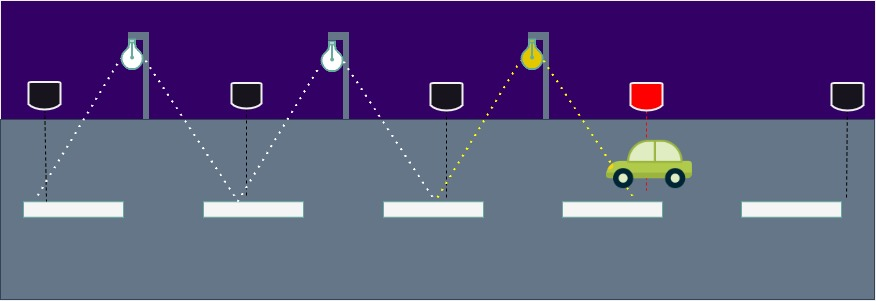
\includegraphics[width=0.9\linewidth,keepaspectratio]{pics/cardraw1.jpg}
    \end{center}
    \caption{Intrare vehicul în sistem}
    \label{fig:car1}
\end{figure}

Trecerea de următorul senzor, prezentată în \figref{fig:car2}, duce la aprinderea următorului felinar, în timp ce nivelul de luminozitate al celui anterior începe să scadă treptat.

 \begin{figure}[!ht]
    \begin{center}
    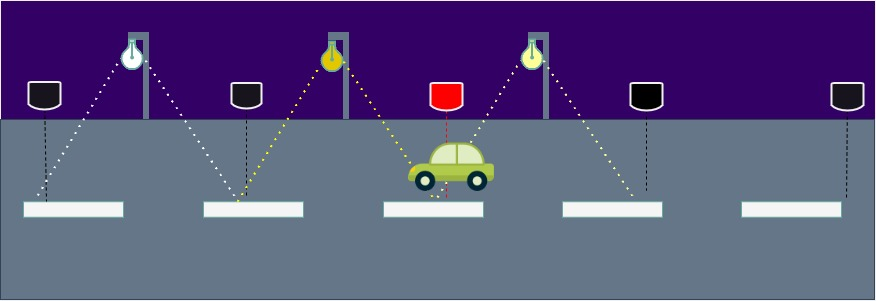
\includegraphics[width=0.9\linewidth,keepaspectratio]{pics/cardraw2.jpg}
    \end{center}
    \caption{Vehicul în stare intermediară}
    \label{fig:car2}
\end{figure}

În \figref{fig:car3} am surprins momentul ieșirii vehiculului din sistem, în care ultimul felinar începe să se stingă, cel anterior încă nu a avut timp să se stingă complet, iar primul deja a revenit la starea inițială.

 \begin{figure}[!ht]
    \begin{center}
    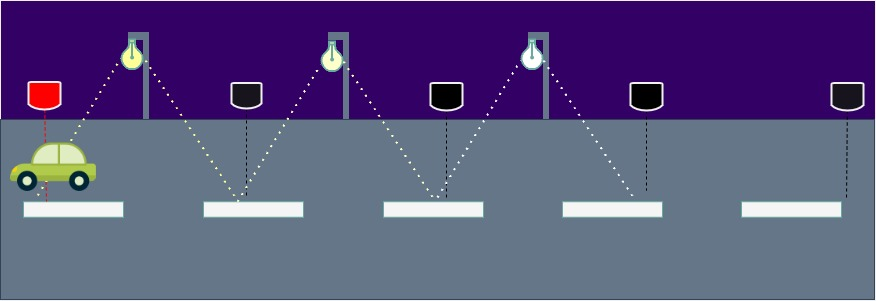
\includegraphics[width=0.9\linewidth,keepaspectratio]{pics/cardraw3.jpg}
    \end{center}
    \caption{Vehicul ieșind din porțiunea reprezentată}
    \label{fig:car3}
\end{figure}

\chapter{Elemente ale arhitecturii hardware}
\label{chap:hard}

\section{Diagrama de context}

Modul de func\c{t}ionare al sistemului este prezentat \^{i}n diagrama de context din   \figref{fig:diag.context}.

\begin{figure}[!ht]
    \begin{center}
    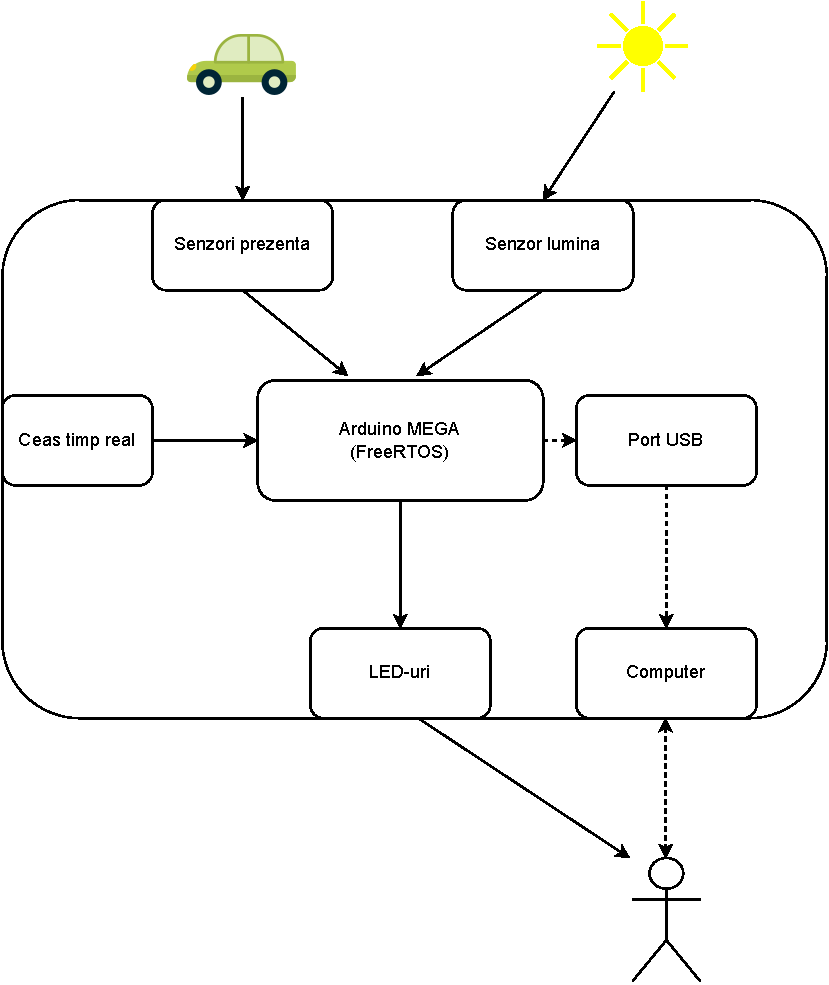
\includegraphics[width=0.7\linewidth,keepaspectratio]{pics/diag_context.drawio.pdf}
    \end{center}
    \caption{Diagrama de context a sistemului în timp real pentru monitorizarea iluminatului public}
    \label{fig:diag.context}
\end{figure}

Componentele sistemului \^{i}n timp real sunt urm\u{a}toarele, conform diagramei de context:

\begin{itemize}
  \item 5 module cu senzor infraroșu; 
\item 3 diode de tip LED;     
 \item Un fotorezistor de tip LDR 5528;
\item  Microcontroller Arduino Mega;
\item  Un ceas în timp real;
\item  Port USB; 
\item Computer.
\end{itemize}

\section{Prezentare elemente diagram\u{a} context}
\subsection{Modul senzor poziție} \label{senzorir}
 Am folosit 5 astfel de module HW-201, ilustrat în \figref{fig:IR1}, pentru detectarea prezenței vehiculelor de pe stradă. Acesta dispune și de un potențiometru, care permite ajustarea razei de detecție a obiectelor la valoarea dorită din intervalul 2-30 cm.

\begin{figure}[!ht]
    \centering
    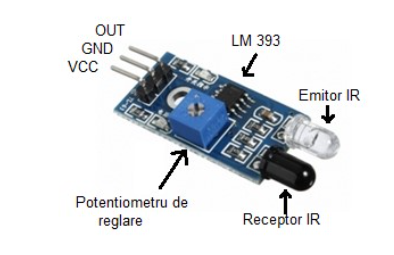
\includegraphics[width=0.4\linewidth,keepaspectratio]{pics/SenzorIR.jpg}
    \caption{Modul infraro\c{s}u}
    \label{fig:IR1}
\end{figure}

Elementul emițător eliberează constant un fascicul de lumină infraroșie, care se reflectă și ajunge la receptor atunci când există un obiect destul de aproape, după cum este prezentat în \figref{fig:IR2}. O mențiune legată de acest mod de funcționare este faptul că, la folosirea a 2 senzori pe părți opuse ale drumului, aceștia trebuie reglați din potențiometru pentru a avea raza de acțiune mai mică decât jumătate din lungimea drumului. În caz contrar, se vor activa reciproc.

\begin{figure}[!ht]
    \centering
    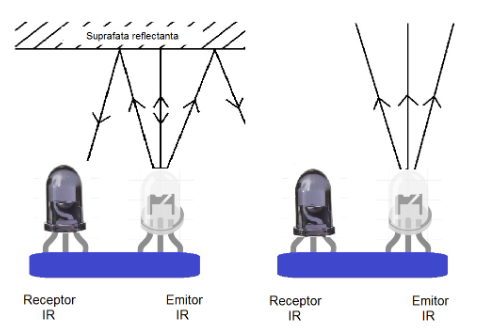
\includegraphics[width=0.6\linewidth,keepaspectratio]{pics/senzorIR2.jpg}
    \caption{Func\c{t}ionare modul infraro\c{s}u}
    \label{fig:IR2}
\end{figure}
O limitare a senzorilor ce se bazează pe detectarea radiațiilor infraroșii este că nu pot fi folosiți pe timp de zi fară a fi influențați negativ de lumina soarelui(e.g. se activează fără nimic în fața lor). Acest lucru nu afectează funcționarea dorită a sistemului, fiind luat în considerare că intrările de la acești senzori sunt citite doar noaptea, ci este doar un inconvenient la realizarea testării pe timp de zi.

În cazurile în care sunt alăturați 2 senzori, distanța dintre aceștia trebuie să fie destul de mare comparativ cu raza de detecție aleasă, pentru a nu permite activarea nedorită a unui senzor de reflecția fasciculului infraroșu al senzorului activat anterior, sau de cel de după el. O altă soluție este acoperirea parțială  a receptorului fiecărui senzor, pentru a permite doar detecția fasciculelor venite de la unghiuri mici, adică de la propriul emițător. 
\subsection{Fotorezistor}

Am ales acest element (\figref{fig:ldr}), pentru a diferenția între momentele când este zi sau noapte. Fotorezistorul este un tip de rezistență ce variază în funcție de gradul de luminozitate aplicat suprafeței acestuia. El este conectat în serie cu o rezistență fixă de 10k$\Omega$, iar valoarea analogică a tensiunii măsurate pe acest rezistor este convertită de Arduino Mega într-un număr natural din intervalul [0,1024]. Compararea acestei valori cu o constantă aleasă arbitrar va determina separarea între cele două moduri de funcționare.

\begin{figure}[!ht]
    \begin{center}
    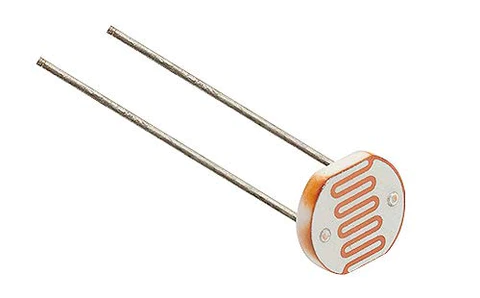
\includegraphics[width=0.3\linewidth,keepaspectratio]{pics/LDR.jpg}
    \end{center}
    \caption{Fotorezistor}
    \label{fig:ldr}
\end{figure}



\subsection{LED-uri}

Am folosit 3 diode de tip LED pentru simularea felinarelor în realizarea proiectului. Am conectat în serie câte o rezistență de 220 $\Omega$ la anodul fiecăreia dintre ele. 

\subsection{Arduino Mega} \label{mega}

Placa de dezvoltare Arduino Mega, ilustrată în \figref{fig:mega}, realizează calculele necesare funcționării corespunzătoare a sistemului. Aceasta dispune și de un ceas în timp real, care va fi util pentru dezvoltarea aplicației folosite. 

\begin{figure}[!ht]
    \begin{center}
    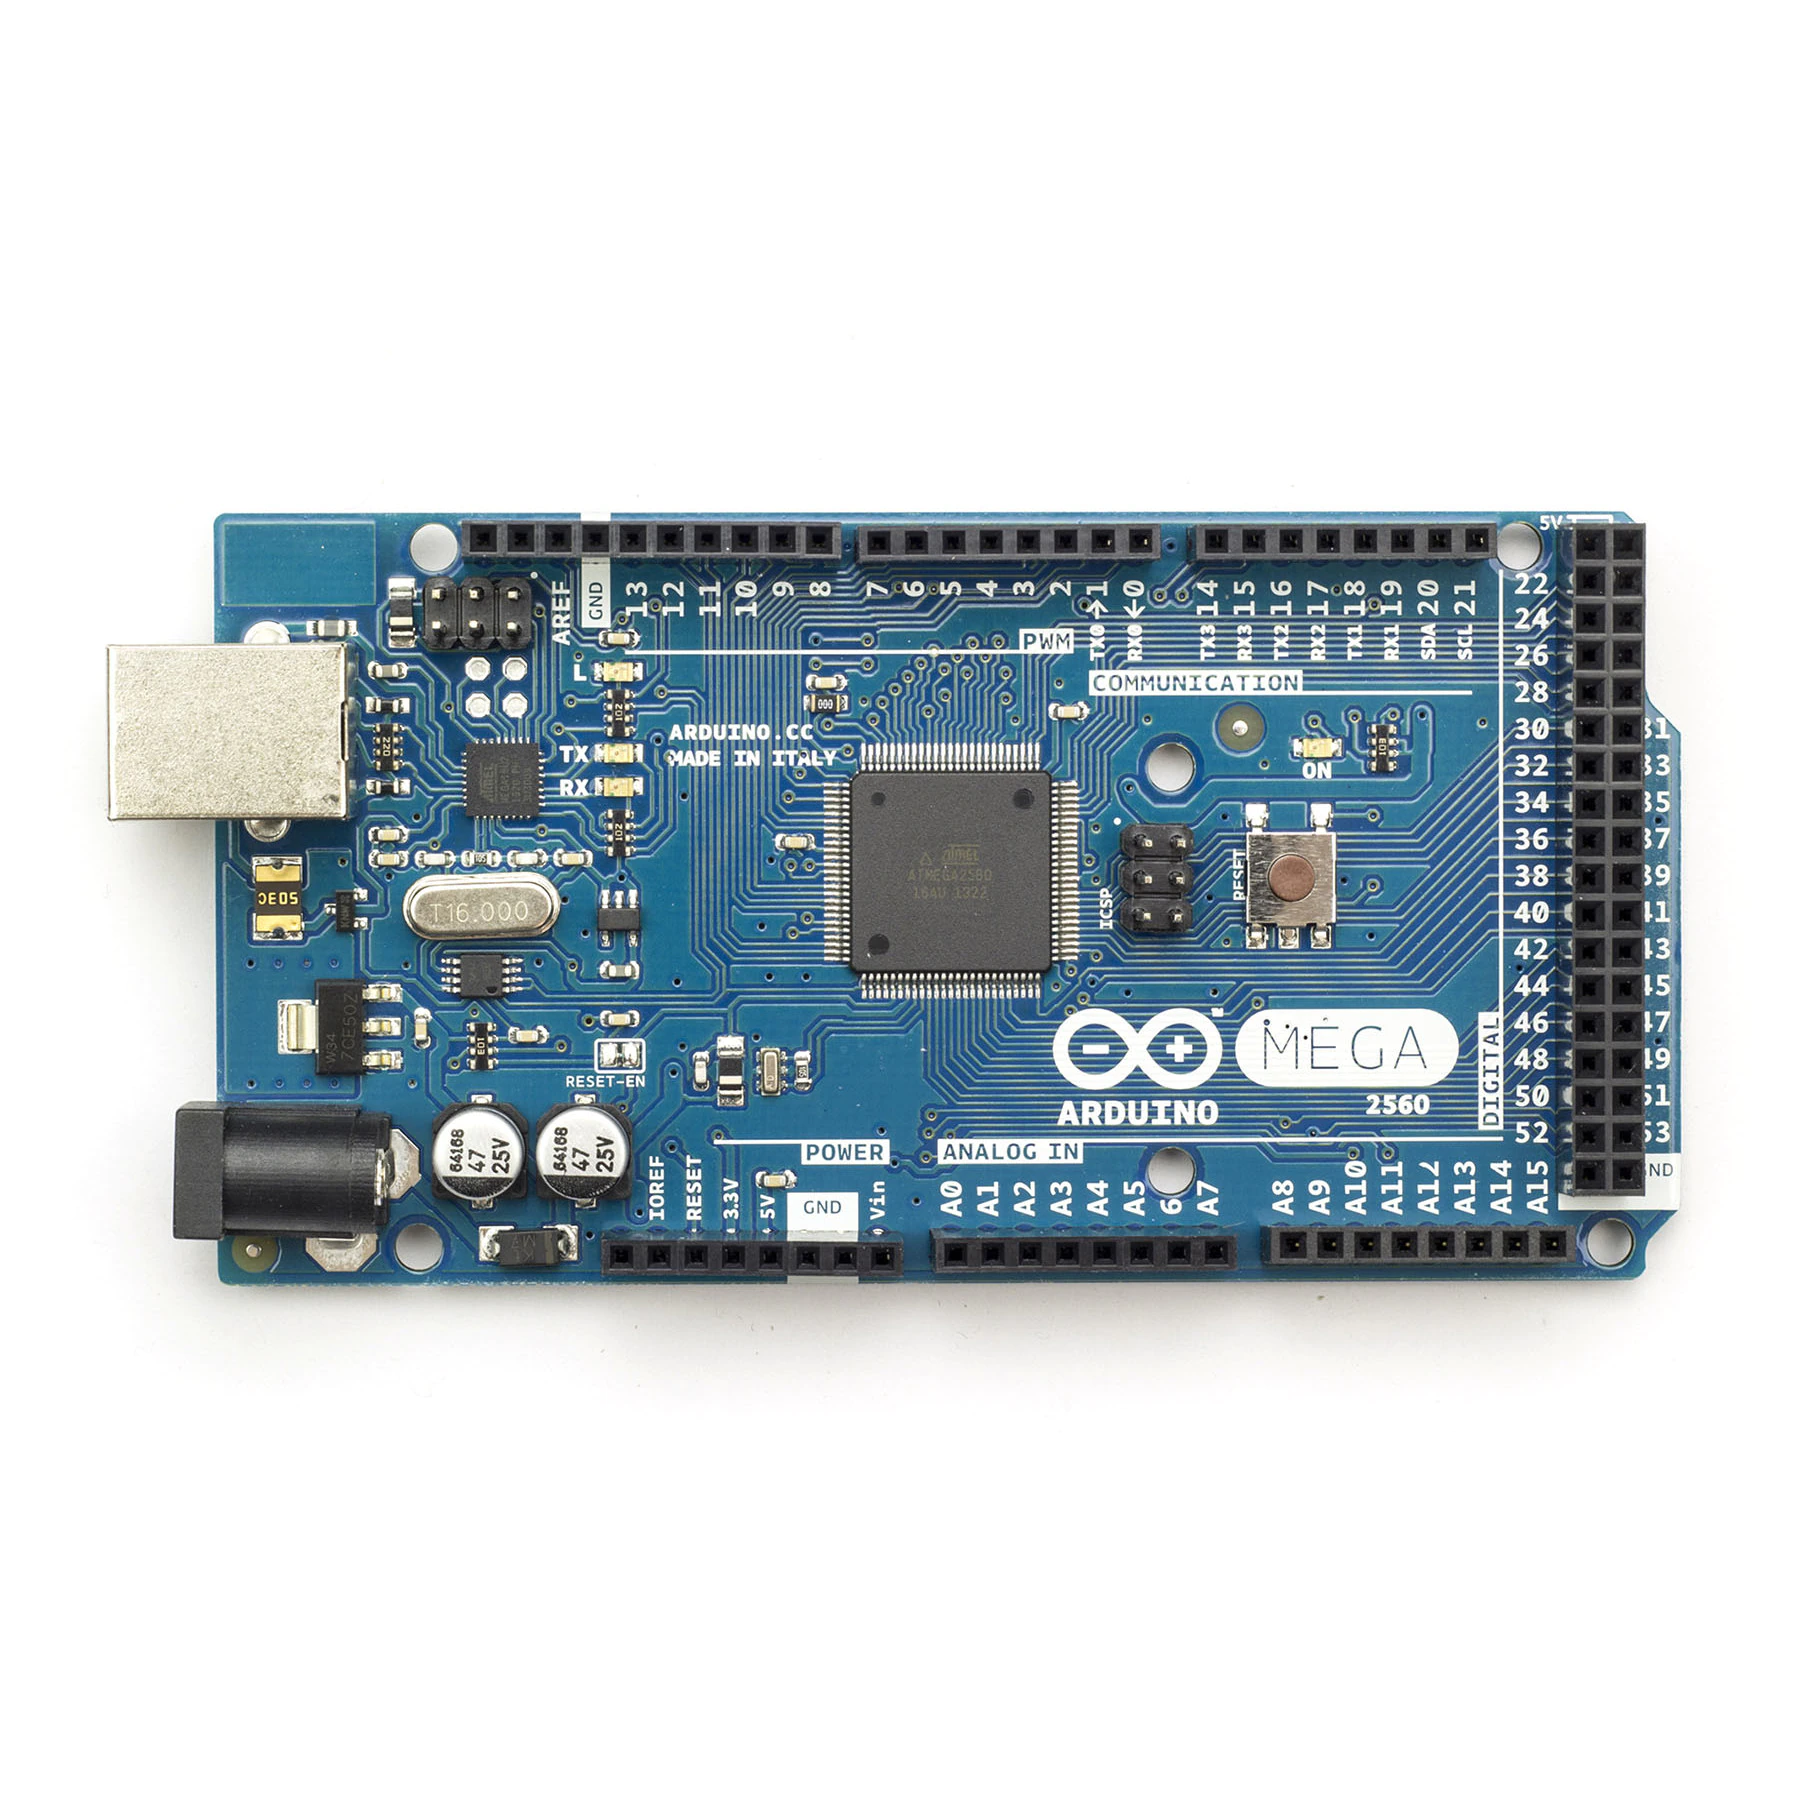
\includegraphics[width=0.5\linewidth,keepaspectratio]{pics/mega.jpg}
    \end{center}
    \caption{Microcontroller Arduino Mega}
    \label{fig:mega}
\end{figure}

Timpul este măsurat cu ajutorul unui ceas oscilator ce generează semnale dreptunghiulare cu frecvența, în cazul unui microcontroller Arduino, de 16MHz. Numărarea repetărilor acestui semnal duce la determinarea cu acuratețe a intervalelor de timp, până la dimensiuni de $\mu$s, conform \cite{Smythe2021.8} .Tot prin microcontroller se realizează și posibila conexiune cu un computer. Cel din urmă nu este strict necesar pentru funcționarea sistemului, dar cu ajutorul său se deschide accesul la citirea de către utilizator a datelor de la senzori și la modificarea codului sursă. Poate fi înlocuit cu o baterie sau altă sursă cu tensiunea recomandată între 7-12V DC.

Deși nu dispune de ieșiri analogice, 15 dintre pinii digitali de pe Arduino Mega permit utilizarea de \gls{pwm}. Această metodă permite transmiterea parțială a curentului la LED-uri, prin mijloace digitale. Alternarea între valori de 0 și 1 creează un semnal dreptunghiular, iar controlul duratei impulsului acesta permite simularea unui semnal analogic \cite{Smythe2021.7}. Această metodă va permite controlul intensității luminii felinarelor.




\section{Simulare a sistemului în Tinkercad și realizarea fizică}



În \figref{fig:arduino} este reprezentată o schemă a modului de conectare a componentelor descrise mai devreme, realizată de mine în Tinkercad. Este de menționat faptul că această platformă nu dispune de toate piesele necesare. Prin urmare, am înlocuit placa Arduino Mega cu un Arduino UNO, iar senzorii de prezență sunt reprezentați printr-o versiune ce dispune doar de receptor. În schimb, modul de conectare va rămâne același și pentru componentele ce au fost schimbate, doar pinii digitali folosiți pentru conectarea senzorilor vor varia față de modelul meu.

\begin{figure}[!ht]
    \begin{center}
    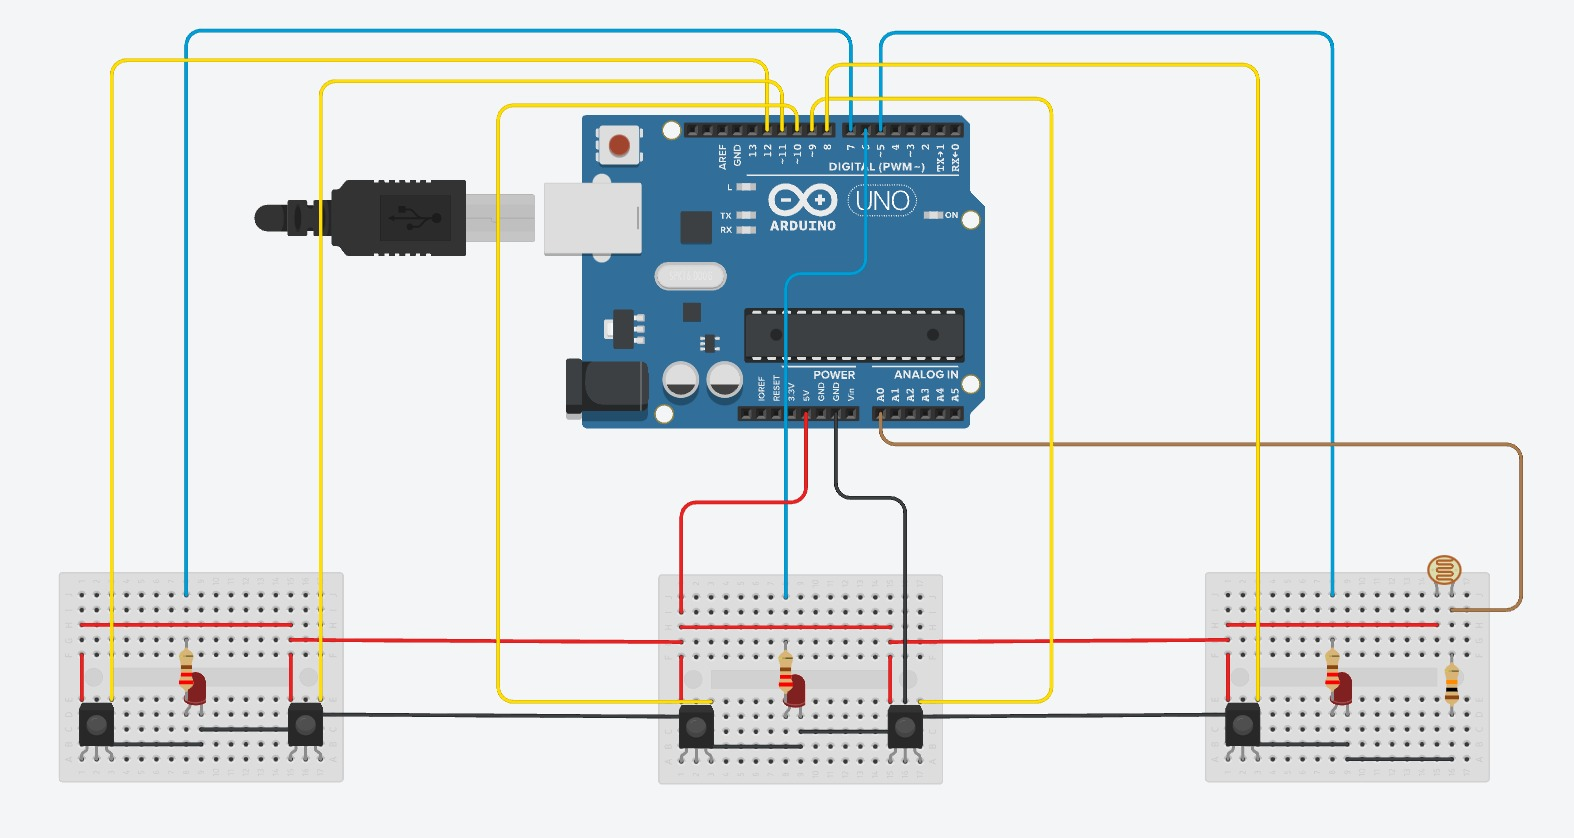
\includegraphics[width=\linewidth,keepaspectratio]{pics/Schema_Arduino.jpg}
    \end{center}
    \caption{Schema sistemului, realizată în Tinkercad}
    \label{fig:arduino}
\end{figure}


Toate componentele sunt conectate la pinul GND, iar senzorii de prezență și fotorezistorul sunt conectați și la pinul de alimentare cu 5V. Citirea datelor se va face pe pinii digitali 49, 50, 51, 52, 53 (8, 9, 10, 11, 12 în \figref{fig:arduino}), de pe Arduino Mega, pentru senzorii de prezență și de la pinul pentru intrări analogice A0 pentru fotorezistor. Intensitatea cu care se vor aprinde LED-urile va fi transmisă pe pinii digitali 5, 6, 7, prin \gls{pwm}.

În \figref{fig:model} este modelul realizat de mine, conform schemei prezentate anterior. Acoperirea   acestuia ajută la blocarea parțială a luminii soarelui la testarea pe timp de zi, iar spațiul lăsat liber permite accesul unui cablu de alimentare la microcontroller. Distanța dintre doi senzori consecutivi este $d=14$cm, egală cu cea dintre 2 felinare consecutive. Poziția fotorezistorului, în partea stângă a modelului, a fost aleasă pentru ca valoarea citită de la acesta să fie influențată cât mai puțin de aprinderea LED-urilor.

\begin{figure}[!ht]
    \begin{center}
    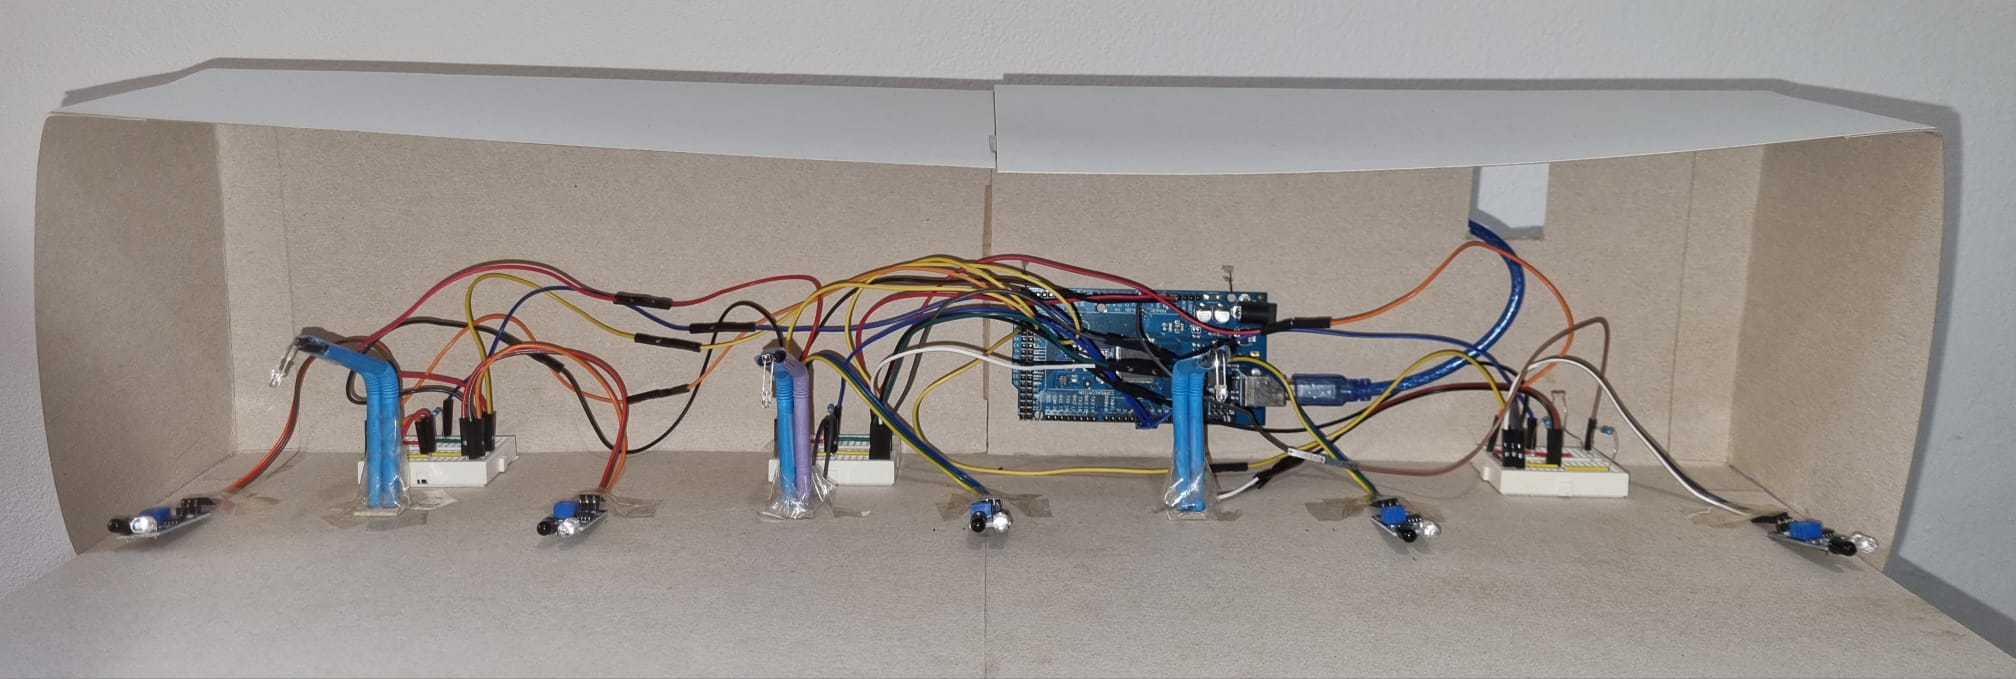
\includegraphics[width=\linewidth,keepaspectratio]{pics/sistemirl.jpeg}
    \end{center}
    \caption{Modelul implementat în realitate}
    \label{fig:model}
\end{figure}
\chapter{Elemente ale arhitecturii software}
\label{chap:soft}

\section{Achizi\c{t}ie date \c{s}i constr\^{a}ngeri de timp} \label{time}

Una dintre caracteristicile principale ale unui sistem în timp real este faptul că acesta trebuie să răspundă schimbărilor venite din mediul înconjurător în limita unui interval de timp, numit \emph{deadline} \cite{str}. Pentru funcționarea corespunzătoare a sistemului, sunt necesare date din 2 surse diferite: senzorii ce detectează prezența unui obiect și senzorul de luminozitate. 

În cazul senzorilor de prezență, este important ca intervalul de timp dintre 2 citiri să fie mai mic decât cel necesar trecerii în întregime a unui vehicul prin fața acestuia. Dacă aș considera suprafața în care senzorii detectează un obiect a fi de lățime neglijabilă,  pot afla viteza necesară pentru ca vehiculul să treacă nedetectat. În crearea programului Arduino după care funcționează sistemul, am observat faptul că intervalul de timp dintre două citiri ale aceluiași senzor este de 15-17 ms (puțin peste 1 tick). 

În exemplul ilustrat în \figref{fig:car4}, am analizat cazul extrem al unei motociclete de lungime relativ mică, 190cm. La convertirea din cm/ms în km/h a rezultat faptul că aceasta ar trebui să atingă o viteză de aproximativ 402km/h pentru a depăși un senzor complet nedetectată.  Prin urmare, frecvența citirilor este suficient de mare pentru a acomoda cerințele sistemului real, și chiar pentru a permite unele modificări aduse cu scopul de a îmbunătăți performanțele sau de a adăuga utilități extra. 

\begin{figure}[!ht]
    \begin{center}
    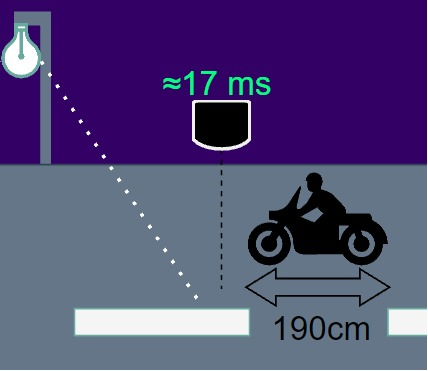
\includegraphics[width=0.5\linewidth,keepaspectratio]{pics/cardraw4.jpg}
    \end{center}
    \caption{Timp citire date}
    \label{fig:car4}
\end{figure}
 Pentru lumină, nu contează atât de mult cât de des se realizează achiziția de date de la senzor, deoarece valoarea citită oricum variază lent. Totuși, și aceasta se va citi la fiecare repetare a task-ului dedicat ei, deoarece trebuie să țină pasul cu citirile senzorilor. Motivul pentru acest fapt este prezentat mai detaliat în \ref{light}.

\section{Descriere FreeRTOS}
Pentru a îndeplini cerințele sistemului în timp real pe care l-am simulat, și aplicația ce determină funcționarea acestuia trebuie să poată folosi concepte specifice programării în timp real \cite{patr}. Este necesară utilizarea firelor de execuție și a semafoarelor pentru a asigura funcționarea în conformitate cu performanțele dorite. De aceea folosirea unui \gls{rtos} este obligatorie. Deși aceasta nu este o caracteristică de bază a Arduino IDE, includerea bibliotecii FreeRTOS permite utilizarea funcțiilor necesare creării și gestiunii firelor de execuție(sub formă de task-uri), a semafoarelor și a mutex-urilor. Această bibliotecă deschide accesul și la funcția vTaskDelay, ce oferă posibilitatea blocării unui anumit task, fără afectarea celorlalte task-uri. Poate fi apelată pentru o durată de timp specificată ori în număr de ticks, ori în milisecunde, prin conversie.

\section{Prezentare task-uri} \label{task}
 În cadrul aplicației am folosit 3 task-uri, ce funcționează după secvența logică din \figref{fig:diag_task-uri}. Ele au aceeași prioritate și se execută în același timp. Ordinea efectuării operațiilor din fiecare task, relativ la celelalte task-uri, este influențată prin incrementarea și decrementarea semafoarelor, unde este necesar.


\begin{figure}[!ht]
    \begin{center}
    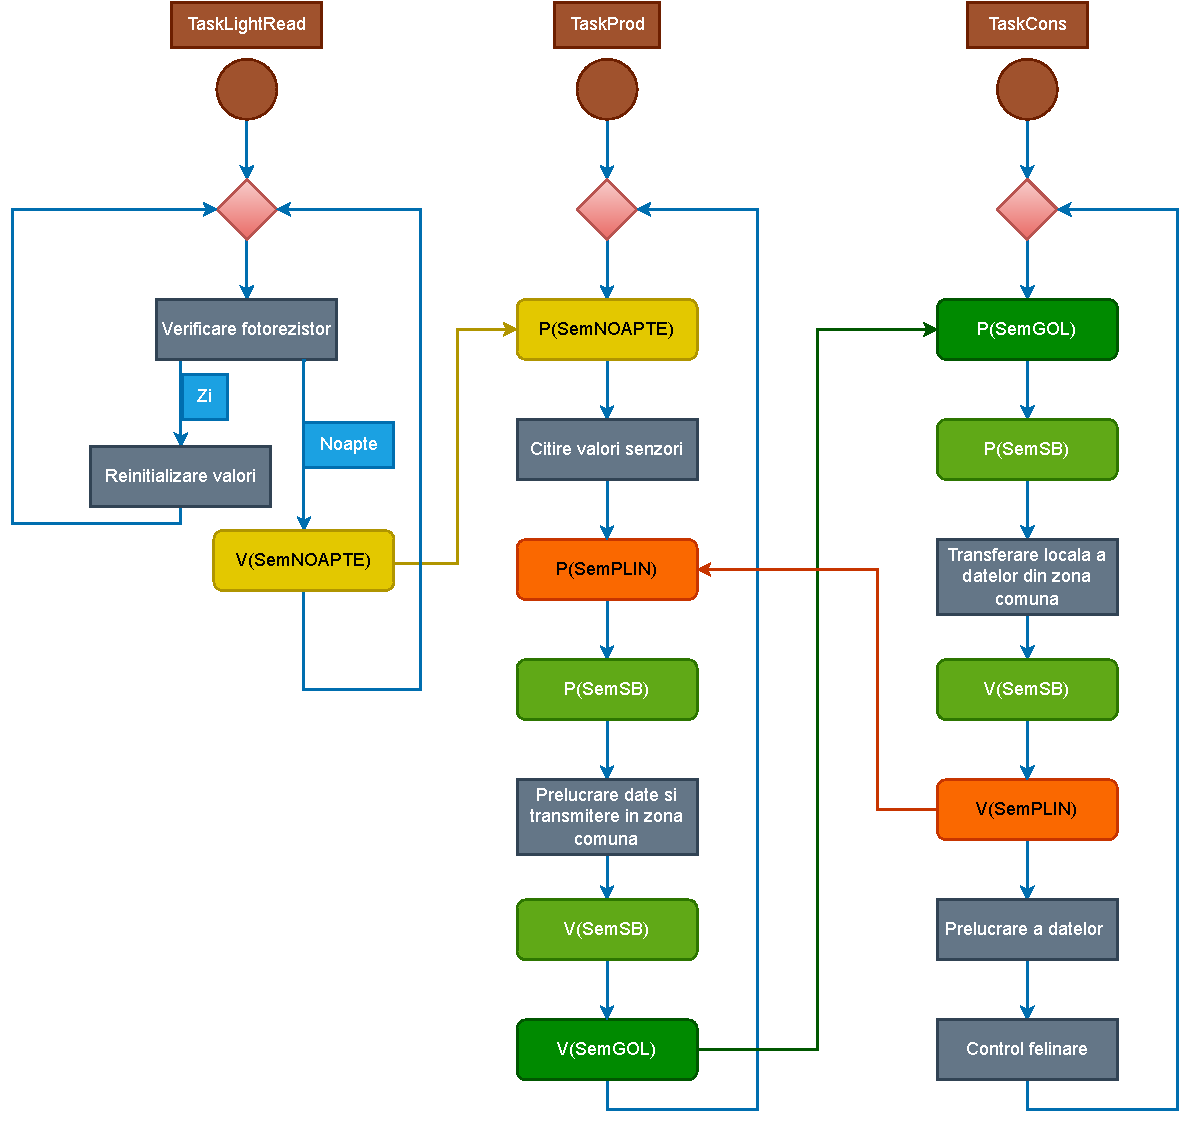
\includegraphics[width=0.9\linewidth,keepaspectratio]{pics/diag.drawio.pdf}
    \end{center}
    \caption{Diagramă task-uri}
    \label{fig:diag_task-uri}
\end{figure}

\subsection{TaskLightRead} \label{light}
 În task-ul acesta (\ref{tlr}) se realizează citirea intrării analogice de pe pin-ul plăcii Arduino la care este conectat fotorezistorul. Dacă valoarea acesteia depășește o anumită constantă, se consideră că afară este zi, urmând reinițializarea tuturor variabilelor folosite la valori nule, pentru a nu rămâne cu cele obținute anterior. Dacă felinarele erau aprinse, sau pe modul de intensitate scăzuta, aici se sting \textbf{complet}. În cazul în care valoarea citită este sub limita impusă, se incrementează semaforul binar SemNOAPTE, cu scopul de a debloca TaskProd.

 Deși acesta este modul normal de funcționare al task-ului, în codul sursă (\ref{tlr}) al aplicației realizate de mine verificarea are loc invers: deblocarea celorlalte două task-uri se întâmplă doar pe timp de zi, pentru ușurarea procesului de testare.
\subsection{TaskProd}
 Acest task producător (\ref{tp}) are rolul de a citi valorile de la senzorii de prezență, lucru care se întâmplă imediat după deblocarea sa, în urma incrementării semaforului SemNOAPTE. Mai departe, la prima rulare, se decrementează semaforul binar SemPLIN, dar se trece, totuși, mai departe, deoarece acesta este inițializat cu valoarea "1". Același lucru este valabil și pentru semaforul pentru secțiunea critică, SemSB, care asigură faptul că zona comună de date nu este accesată simultan de mai multe task-uri \cite{patr}. În urma alterării și transferării noilor date, acesta este deblocat. Apoi, semaforul binar SemGOL este incrementat, pentru deblocarea task-ului TaskCons. La rulări ulterioare ale task-ului, acesta se va bloca fie în SemNOAPTE, dacă s-a făcut zi, sau în SemPLIN, dacă nu a fost incrementat din TaskCons. 
\subsection{TaskCons}
 Deblocarea task-ului consumator (\ref{tc}) are loc la incrementarea în TaskProd a semaforului SemGOL. Urmează trecerea datelor din zona comună în plan local, facilitată de semaforul SemSB. În urma incrementării lui SemPLIN, ce permite deblocarea lui TaskProd, are loc prelucrarea datelor obținute și controlul felinarelor conform condițiilor impuse. În final, task-ul se repetă, în concordanță cu toate cele menționate pană acum.
\section{Analiz\u{a} a codului}

 În această secțiune voi menționa și descrie câteva fragmente mai importante din codul sursă, cu scopul de a oferi o privire mai clară asupra modului de funcționare al aplicației. Toate variabilele scalare sau vectoriale vor fi inițializate în întregime cu 0, cu excepția unora dintre semafoare, conform Secțiunii \ref{task}. Constanta $d$ reprezintă distanța (în cm) dintre 2 senzori consecutivi și este egală cu 14. În cazul buclelor for, acestea în general se repetă de $n = 5$ ori dacă sunt folosite valorile corespondente senzorilor de prezență, sau de $n - 1 = 4$ ori, pentru operații ce influențează calculul sau afișarea vitezei pe o anumită porțiune de drum.

\subsection{Prelucrare date citite și counter obiecte} \label{counter}
\indent \indent 
Modulele cu senzor infraroșu folosite pot avea ca ieșiri valorile "1", când nu se află nimic în fața lor, sau "0", când au un obiect în față. Aceste valori numerice nu ajută foarte mult, deoarece scopul  este de a obține viteza vehiculului. De aceea va fi utilizată funcția millis() din Arduino IDE, pentru a obține  timpul (în ms) trecut de la momentul rulării aplicației până la activarea unui senzor.

În următorul fragment de cod este prezentată zona de \emph{Prelucrare date și transmitere în zona comună} din TaskProd. În aplicația realizată de mine, drumul este împărțit în n-1 porțiuni egale ca dimensiune, aflate între cei n senzori de prezență folosiți.

\begin{verbnobox}[\verbarg]
     for(int in = 0; in < 5; in ++){
        if (f[in] == 1){
          b[in]= bn[in];
          bn[in] = 0;
          f[in] = 2;
        }
        if (aux[in] - bc[in] == 1) {
            if (in <= 3) {
              c[in] ++;
            }
            if ((in >= 1) && c[in-1]>0){
              c[in - 1] --;
             if ((bn[in-1] != 0) &&(c[in - 1] == 1)){
                  f[in-1] = 1;
               } 
           }      
            if (in == 4)
              b[in] = millis();
            else if ((in <= 3) && (c[in] == 1)){ 
                  b[in] = millis();
            }
            else if ((in <= 3) && (c[in] > 1)){
                bn[in] = millis();
            }
         }
          aux[in] = bc[in];      
      }   
\end{verbnobox}

Numărul de vehicule de pe fiecare porțiune de drum este salvat în vectorul counter $\mathbf{c[n - 1]}$, iar acesta este actualizat la fiecare depășire a unuia dintre senzori de un vehicul. Este important ca atât modificarea valorii din $\mathbf{c}$, cât și cea a momentului de timp înregistrat, să se întâmple o singură dată la fiecare activare a unui senzor de prezență. Pentru a îndeplini această cerință cu acuratețe, trebuie recunoscute doar momentele când un obiect apare în fața unui senzor, sau, mai precis, când valoarea citită de la senzor se transformă din "1" în "0". Vectorul $\mathbf{bc[n]}$ conține valorile obținute în secțiunea de Citire valori senzori, iar egalarea elementelor din $\mathbf{aux[n]}$ la finalul buclei for face ca la următoarea execuție a task-ului să pot compara valoarea actuală cu cea citită cu un pas în urmă. Diferența dintre cele două poate fi egală cu 1 doar în cazul dorit, cel în care $\mathbf{aux[in]}=1$ și $\mathbf{b[in]}=0$. În cazul unui singur vehicul,  momentul la care a fost activat un senzor este salvat în $\mathbf{b[n]}$. Am adăugat variabilele vectoriale $\mathbf{f[n]}$ și $\mathbf{bn[n]}$, pentru tratarea cazului în care mai multe vehicule se află pe aceeași porțiune de drum. Un exemplu al unei astfel de situații este reprezentat în \figref{fig:doi1} și \figref{fig:doi2} .
\begin{figure}[!ht]
    \begin{center}
    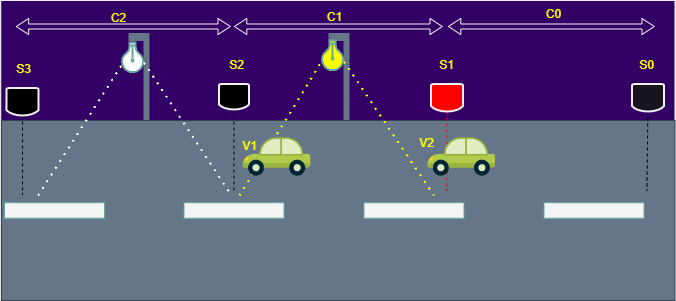
\includegraphics[width=0.7\linewidth,keepaspectratio]{pics/doi1.png}
    \end{center}
    \caption{Situație 2 vehicule pe aceeași porțiune de drum, moment 1}
    \label{fig:doi1}
\end{figure}

\begin{figure}[!ht]
    \begin{center}
    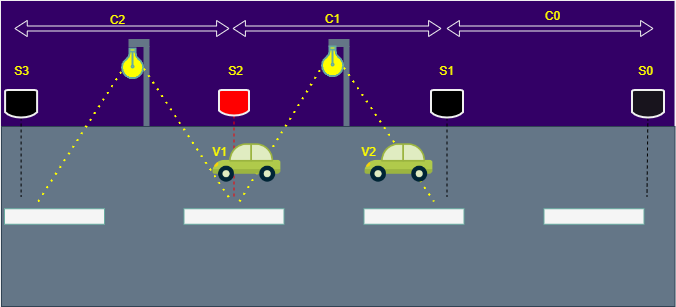
\includegraphics[width=0.7\linewidth,keepaspectratio]{pics/doi2.png}
    \end{center}
    \caption{Situație 2 vehicule pe aceeași porțiune de drum, moment 2}
    \label{fig:doi2}
\end{figure}

În această situație, comportamentul aplicației pe porțiunea de cod descrisă este următorul:
\begin{enumerate}
\item  La depășirea senzorului S1 de vehiculul V2, counter-ul $\mathbf{c[1]}$ este incrementat și are valoarea 2. Momentul de timp este salvat în vectorul $\mathbf{bn[1]}$.
\item  La activarea lui S2, momentul este salvat în $\mathbf{b[2]}$, iar flag-ul $\mathbf{f[1]}$ primește valoarea 1.
\item  La următoarea execuție a task-ului, acest flag indică faptul că valoarea din $\mathbf{b[1]}$ nu mai este necesară, deoarece a fost folosită deja în calculul unei viteze. Ea va fi înlocuită cu valoarea din $\mathbf{bn[1]}$, iar $\mathbf{f[1]}$ va deveni 2. În această stare, el indică faptul că următorul calcul al vitezei cu noul $\mathbf{b[1]}$ este doar unul intermediar și nu va influența luminozitatea felinarelor.   

\end{enumerate}

Această metodă de implementare acoperă și cazul apariției unui vehicul V3 în porțiunea C1, înaintea ieșirii lui V2 din aceasta, prin eliberarea lui $\mathbf{bn[1]}$ pentru trecerea lui V3 prin S1. Modelul realizat funcționează doar până la limita de 2 vehicule existente simultan în aceeași porțiune. Pentru generalizare, vectorul $\mathbf{bn}$ ar trebui să fie o matrice de $n$ coloane și $m$ linii, unde $m$ este un număr natural, cu 1 mai mic decât numărul de automobile maxime admise într-o porțiune a drumului, ales în funcție de lungimea porțiunii respective.


\subsection{Transmitere date între task-uri}
 Pentru folosirea datelor primite de la senzorii de prezență, este necesar transferul între task-uri prin folosirea unor vectori declarați global, astfel:

\begin{verbnobox}[\verbarg]
for (int i = 0; i < 5; i ++) { 
      z[i] = b[i];
      zn[i] = bn[i];
    }
\end{verbnobox}


\subsection{Transformare date senzori mișcare în valori de timp \c{s}i \^{i}n vitez\u{a}}
Pentru aflarea vitezei, se scad momentele de timp la care au fost activați 2 senzori consecutivi și se realizează transformarea prin calcule matematice, în funcție de unitatea de măsură dorită că rezultat. În cazul meu, conversia este din cm/ms în km/h. Diferențierea între valorile lui $\mathbf{c}$ ale secțiunii în care intră vehiculul se face pentru a determina dacă valoarea de timp corespondentă acestuia trebuie luată din $\mathbf{z}$ sau $\mathbf{zn}$. Deși viteza este calculată la fiecare rulare a task-ului în $\mathbf{vint[n-1]}$vint, aceasta este salvată în $\mathbf{v[n-1]}$ și afișată doar la momentul activării unui senzor, numai în situațiile în care flag-ul $\mathbf{f}$ nu este egal cu 2. Dacă acesta este 2, va fi reinițializat cu 0. În $\mathbf{auxv[n-1]}$ este salvată valoarea vitezei intermediare la execuția anterioară a task-ului, pentru comparare cu cea actuală, similar cu $\mathbf{aux}$ în \autoref{counter}.

\begin{verbnobox}[\verbarg]
for (int i = 0; i < 4; i ++) {
      if (i==3)
        t[i] = z[i + 1] - z[i];
      else if (c[i + 1] == 1)
        t[i] = z[i + 1] - z[i];
      else if (c[i + 1] == 2)
        t[i] = zn[i + 1] - z[i];
      
      if (t[i] != 0)
        vint[i] = 10*d * 3.6/((float)t[i]);
      else if (t[i] == 0) 
        vint[i] = 0;
      if (auxv[i] != vint[i]){
        if ((f[i] != 2)&&(vint[i]>=0)){
          v[i] = vint[i];
          Serial.print ... 
        }
        else {
          Serial.print ...
          f[i] = 0;
        }
      }  
      auxv[i] = vint[i];
      ...
   }
\end{verbnobox}




\subsection{Control nivel intensitate lumină}

 Pentru controlul intensității luminii, este folosită o abordare bazată pe \gls{pwm}. Aceasta permite folosirea ieșirilor digitale corespondente LED-urilor, pe post de ieșiri analogice (\autoref{mega}), convertite din valori numerice aparținând intervalului [0,255]. Aceste valori sunt păstrate în vectorul $\mathbf{lum[n-2]}$, și sunt influențate de viteza calculată a vehiculelor, astfel:

\begin{verbnobox}[\verbarg]
    for (int i = 0; i < 4; i ++) {
      ...
      if (i > 0){ 
        if (lum[i - 1] < 3)
          lum[i - 1] = 3;
        if ((c[i] == 0) && ( lum[i - 1] > 3)) {
            if (timp == 0) {
              if (lum[i - 1] > 8)
                lum[i - 1] = lum[i - 1] * 0.7;
              else
                lum[i - 1] --;
            }
            timp ++;
            timp = timp % 5;      
        }
        else if (c[i] == 0) {     
        }
        else if (c[i] == 1){
          if (v[i-1] > 4){ 
            lum[i - 1] = 255;      
          }
          else if (v[i-1] > 1){ 
             if (lum[i - 1] > 150)
               lum[i - 1] =  lum[i - 1] - 2;
             else 
               lum[i - 1] = 150;
          }           
          else if (v[i - 1] > 0){ 
             if (lum[i - 1] > 40)
               lum[i - 1] =  lum[i - 1] - 2;
             else 
               lum[i - 1] = 40;
          }
         }
         else if (c[i] == 2){
          if ((v[i - 1] > 4)&& (lum[i - 1] < 150)){ 
            lum[i - 1] = 255;      
          }
          else if ((v[i - 1] > 1) && (lum[i - 1] < 150)){ 
            lum[i - 1] = 150;
          }           
         }  
         analogWrite(4 + i, lum[i - 1]);
        }
   }
\end{verbnobox}
 LED-urile primesc ca ieșire valoarea aflată în $\mathbf{lum}$, în cazul în care valoarea counter-ului $\mathbf{c}$ corespondent porțiunii lor de drum este diferită de 0. Când aceasta devine iar 0 (atunci când nu se mai află niciun vehicul în raza felinarului), valoarea din $\mathbf{lum}$ începe să scadă treptat, până devine 3. Valorile din $\mathbf{lum}$ se schimbă doar la modificări aduse lui $\mathbf{v}$, iar valorile din $\mathbf{vint}$ nu au niciun efect asupra lor.
 
 Diferențierea dintre cazurile în care $\mathbf{c[i]}=1$ și $\mathbf{c[i]}=2$ se face pentru a asigura faptul că este oferită o prioritate mai mare vehiculelor cu viteze mai mari, la stabilirea intensității felinarelor. Pentru momentul 1 al exemplului descris în \autoref{counter} (\figref{fig:doi1}), trecerea lui V2 prin fața lui S1 va determina schimbarea intensității luminii felinarului doar dacă viteza acestuia este mai mare decât viteza pe care a avut-o V1 la trecerea prin S1. În cazul contrar, valoarea din $\mathbf{lum}$ va începe să scadă treptat doar la ieșirea lui V1 din porțiunea C1, la momentul 2(\figref{fig:doi2}).

\chapter{Moduri alternative de funcționare și cazuri speciale}
\label{chap:extra}

 După cum am menționat în \autoref{time}, frecvența citirilor senzorilor de prezență este principalul factor ce limitează numărul de posibilități ale sistemului. În modelul prezentat, fiind o versiune la scară mult redusă, frecvența citirilor aduce două probleme principale:

\begin{enumerate}
\item Obiectele folosite pentru a simula vehiculele devin mult mai scurte;

\item Distanțele mai mici între senzori duc la calcule eronate în cazul obiectelor cu viteze mari. 

\end{enumerate}

 Sistemul real permite scăderea frecvenței citirilor, fară a ieși din limitele performanțelor dorite, în schimbul adăugării unor caracteristici suplimentare.

 \section{Ecran LCD}

\indent \indent Sistemul permite adăugarea unui  \gls{lcd}, ce permite observarea anumitor date intermediare(e.g. viteza unui vehicul în fiecare zonă a sistemului), fară a fi necesară conectarea la computer. Acesta folosește un modul I2C și se conectează la 5V și GND împreună cu restul componentelor, iar adițional, la pinii dedicați SDA și SCL de pe Arduino Mega.

\begin{figure}[!ht]
    \begin{center}
    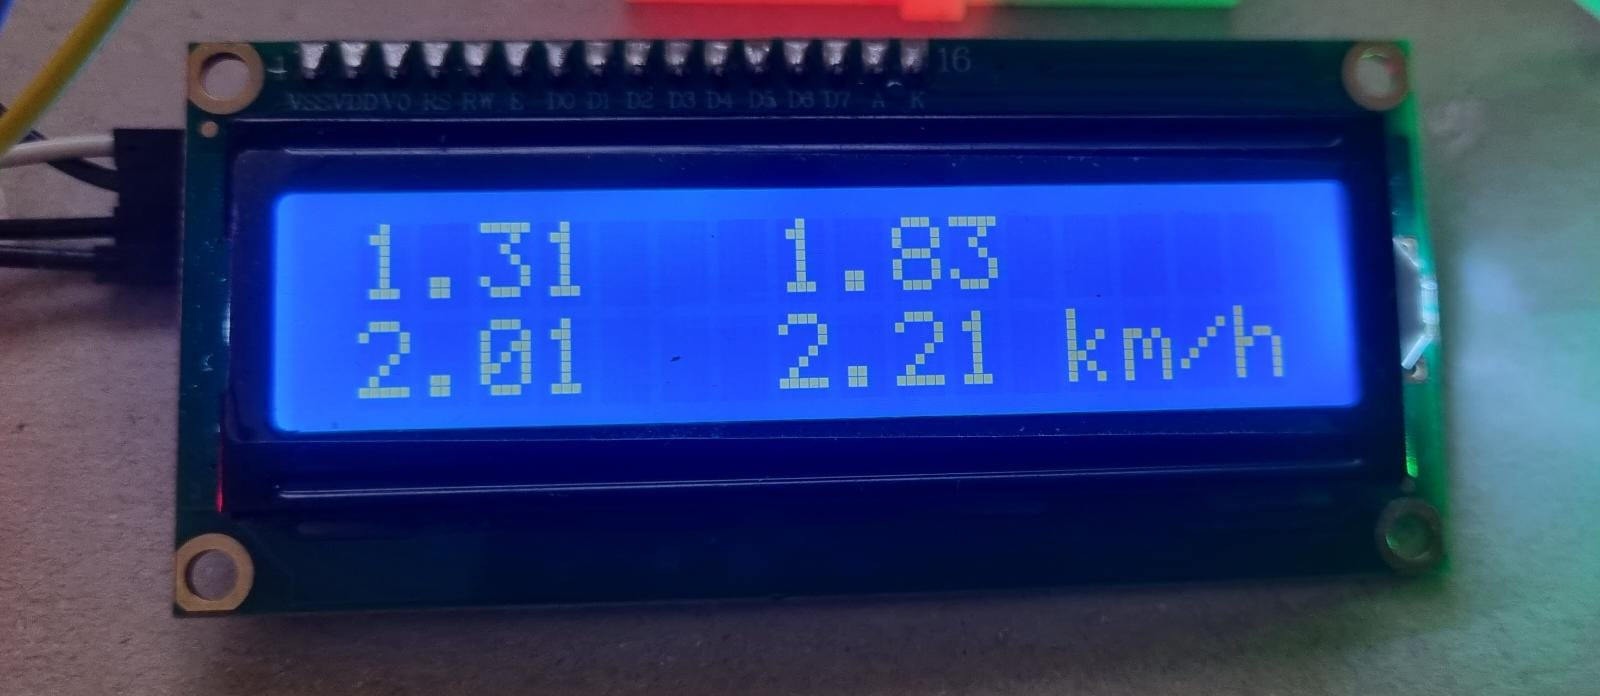
\includegraphics[width=0.5\linewidth,keepaspectratio]{pics/LCD.jpg}
    \end{center}
    \caption{LCD}
    \label{fig:LCD}
\end{figure}


 Pentru utilizarea \gls{lcd}-ului, este nevoie de un task suplimentar (\ref{tlcd}) ce se ocupă cu gestiunea acestuia. Incrementarea semaforului binar SemLCD are loc în TaskProd, la schimbarea oricărei dintre viteze. Acest lucru asigură funcționarea corectă a programului și oprește rescrierea datelor de pe \gls{lcd} la fiecare execuție a task-ului. Astfel, acestea sunt rescrise doar când apare o schimbare. Verificarea și incrementarea valorii variabilei $p$ are loc pentru a asigura faptul că inițializarea display-ului se întâmplă doar la prima rulare a task-ului, ilustrat în \figref{fig:tasklcd}.

  \begin{figure}[!ht]
    \begin{center}
    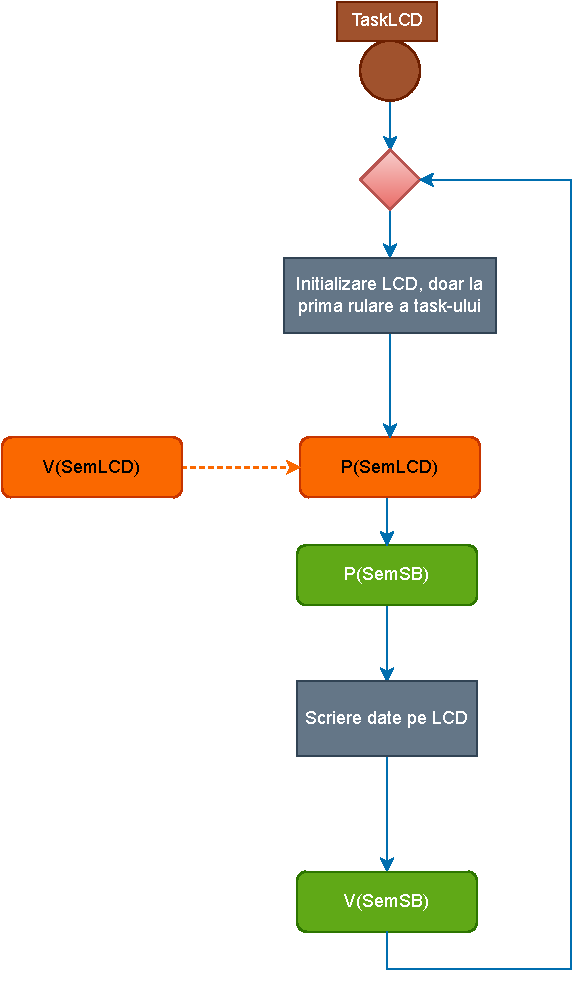
\includegraphics[width=0.6\linewidth,keepaspectratio]{pics/TaskLCD.drawio.pdf}
    \end{center}
    \caption{TaskLCD}
    \label{fig:tasklcd}
\end{figure}

Prezența și funcționarea acestuia necesită sincronizări adiționale între task-uri și un mic delay adăugat la citirile senzorilor. La încercarea rulării în starea inițială, simpla scriere pe LCD bloca tot programul. În cazul soluției găsite de mine pentru rezolvarea problemei, intervalul de timp dintre două citiri a ajuns să fie aproximativ dublu, în jur de 33-34ms.

\section{Citire pe porțiuni a senzorilor} \label{part}

O versiune alternativă a aplicației pentru sistemul de iluminat în timp real este cea în care fiecare senzor este citit individual, într-o rulare a task-ului TaskPROD, iar în TaskCONS se calculează doar o singură viteză, cu ajutorul valorii de timp primite la momentul actual și cea de la execuția anterioară a task-ului. Această metodă este ușor de generalizat. Modificările necesare pentru extinderea sistemului constau în schimbarea dimensiunii buffer-ului din zona comună de date și a transformării semafoarelor binare SemPLIN și SemGOL din \figref{fig:diag_task-uri} în semafoare generalizate. Atât dimensiunea vectorului de date, cât și a semafoarelor va deveni egală cu numărul nou de senzori de prezență \cite{patr}.

În schimb, aici se întâlnește problema scăderii frecvenței citirilor. La citirea unui singur senzor la fiecare rulare a lui TaskCONS, intervalul de timp dintre două citiri ale aceluiași senzor se multiplică cu $n$, unde $n$ este egal cu numărul senzorilor de prezență. Astfel, citirile se realizează la fiecare aproximativ 85ms, în loc de cele 17ms necesare inițial. Acest lucru nu numai că face viteza necesară pentru ca un vehicul să treacă neobservat de $n$ ori mai mică decât cea calculată în \autoref{time}, dar duce și la calcularea greșită a vitezei vehiculului.

În \figref{fig:speed} este reprezentat un exemplu de calcul al vitezei cu citirile aceluiași senzor la un interval de 85 ms, după cum arată variația variabilei t. În acest caz, este calculată viteza $\mathbf{v[0]}$, iar distanța dintre 2 senzori este destul de mică(20cm) pentru a se obține valori foarte mici pentru $t$(variabilă scalară pentru modalitatea de implementare din această secțiune). Viteza se calculează prin împărțire la $t$, ceea ce înseamnă că diferențele mari între valorile sale, relativ la el însuși, duc la obținerea unui rezultat ce nu reflectă realitatea. În exemplul prezentat, asta înseamnă că $\mathbf{v[0]}$ va fi afișat ca 42.35 km/h pentru orice viteză mai mare sau egală cu acest număr, 7.06km/h pentru orice valoare din intervalul [7.06, 42.35) ș.a.m.d.

  \begin{figure}[!ht]
    \begin{center}
    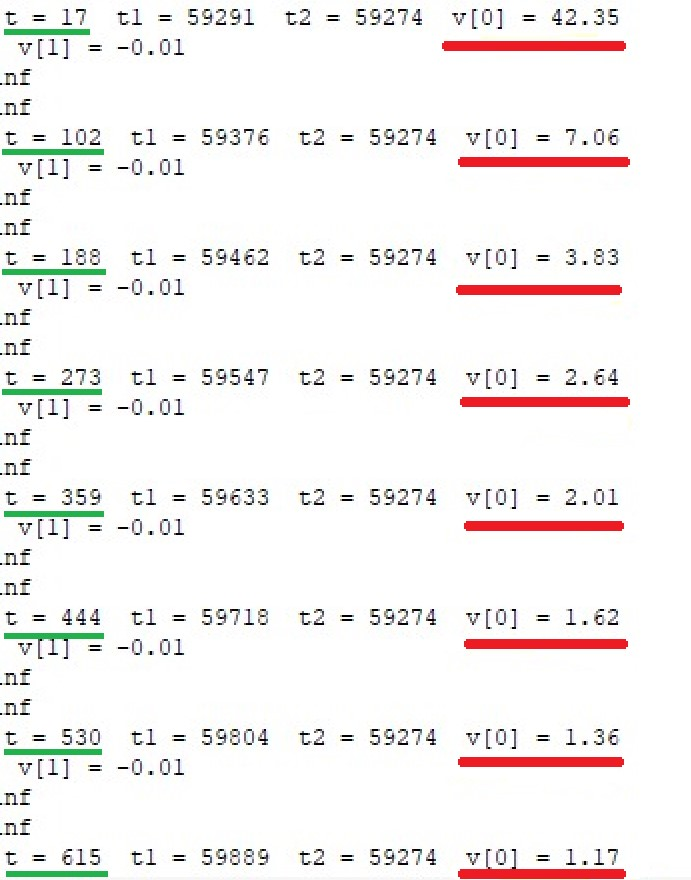
\includegraphics[width=0.585\linewidth,keepaspectratio]{pics/speed.jpg}
    \end{center}
    \caption{Calcul eronat al vitezei}
    \label{fig:speed}
\end{figure}


\subsection{Analiză rezultate} \label{fail}

Rezultatele de pe Serial Monitor, din \figref{fig:speed} pot fi observate și în \figref{fig:v1}, sub formă de grafic. 

\begin{figure}[!ht]
    \begin{center}
    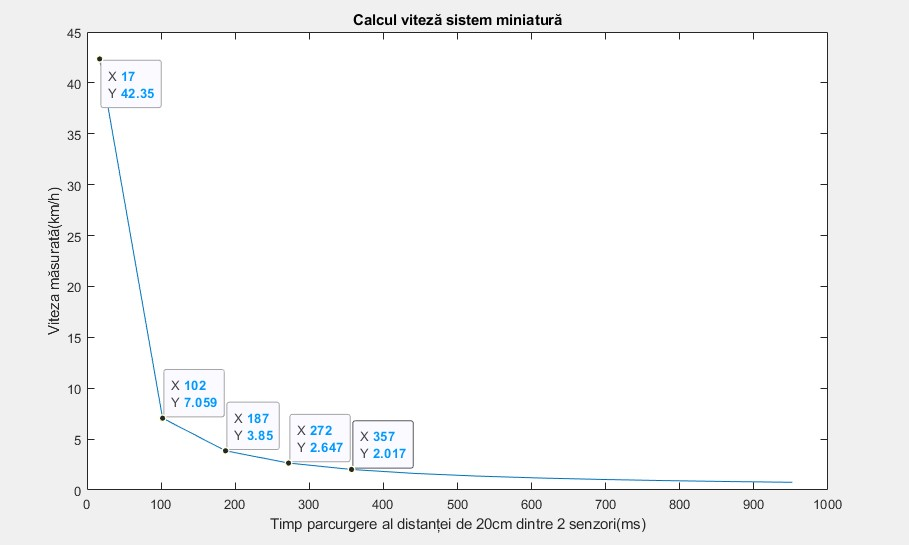
\includegraphics[width=0.9\linewidth,keepaspectratio]{pics/v1.jpg}
    \end{center}
    \caption{Comportarea sistemului mod 1: distanța între senzori 20 cm}
    \label{fig:v1}
\end{figure}

În \figref{fig:v2} am realizat același calcul al vitezei, la modificarea distanței dintre senzori la 35m, în concordanță cu sistemul real. Forma graficului rămâne aceeași, iar singura diferență este creșterea valorii vitezei, direct proporțional cu distanța. 

\begin{figure}[!ht]
    \begin{center}
    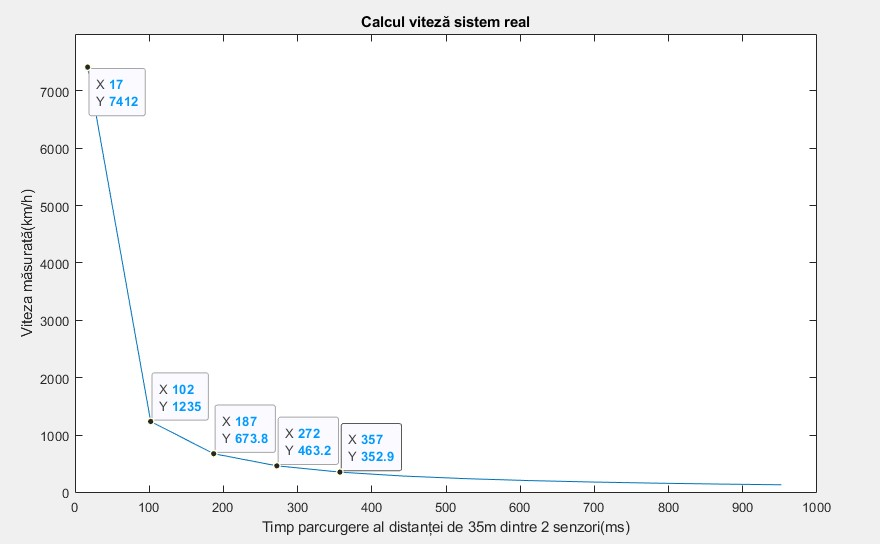
\includegraphics[width=0.9\linewidth,keepaspectratio]{pics/v2.jpg}
    \end{center}
    \caption{Comportarea sistemului mod 2: distanța între senzori 35 m}
    \label{fig:v2}
\end{figure}

În schimb, dacă extind graficul până la momentele de timp în care viteza ar avea valori mai realiste pentru un automobil, ca în \figref{fig:vmare} și \figref{fig:vmic}, se poate observa cum eroarea maximă posibilă, egală cu diferența între două viteze consecutive de pe grafic, începe să scadă. 

\begin{figure}[!ht]
    \begin{center}
    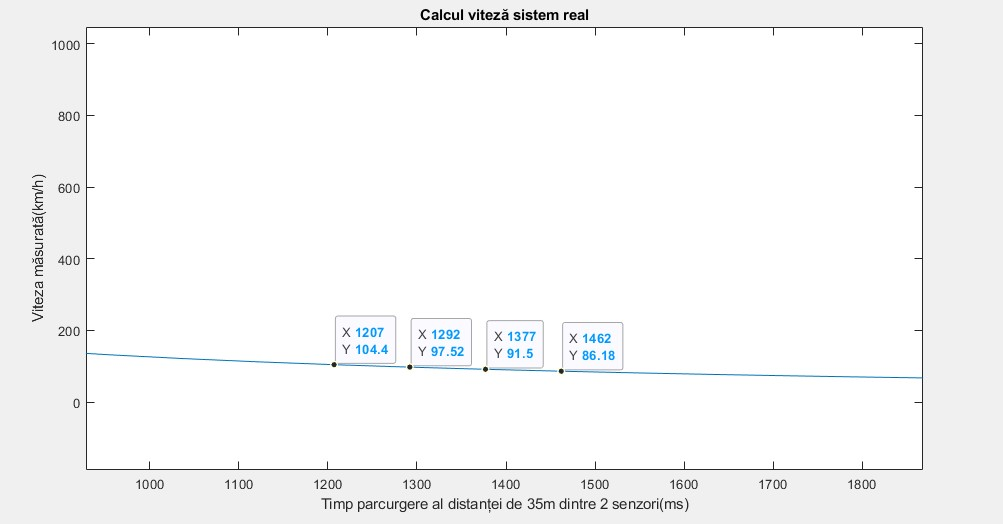
\includegraphics[scale = 0.5]{pics/vmare.jpg}
    \end{center}
    \caption{Eroare posibilă la viteze mari}
    \label{fig:vmare}
\end{figure}

\begin{figure}[!ht]
    \begin{center}
    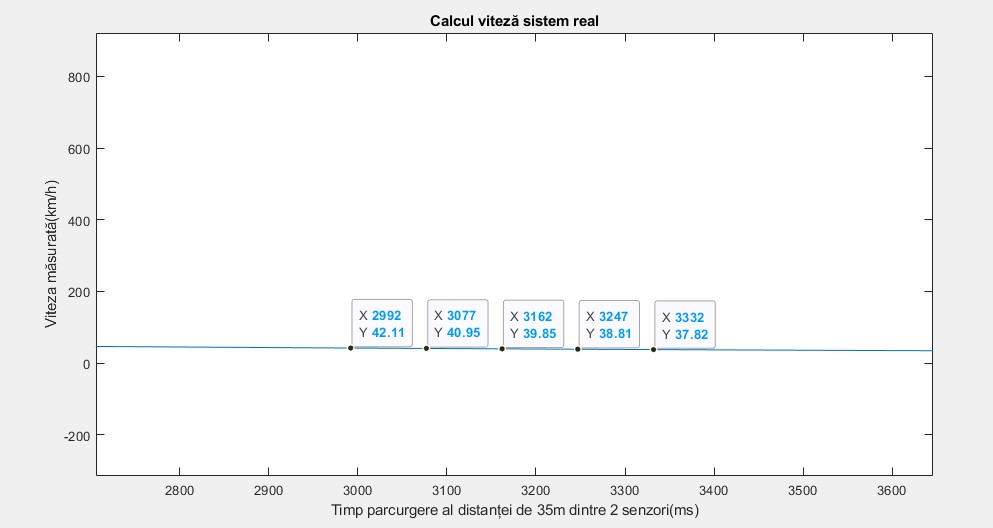
\includegraphics[scale = 0.5]{pics/vmic.jpg}
    \end{center}
    \caption{Eroare posibilă la viteze mici}
    \label{fig:vmic}
\end{figure}

În concluzie, eroarea maximă posibilă pentru măsurarea vitezei devine din ce în ce mai mică, la scăderea vitezei obiectului observat, iar acest proces poate fi grăbit prin mărirea distanței dintre senzori. Astfel, aceste valori pot fi ajustate pentru un sistem de iluminare publică, în funcție de intervalul numeric în care poate fi încadrată viteza vehiculelor pe acea porțiune de drum.

\section{Colectare date valori viteză} \label{collect}

Din moment ce sistemul, în starea sa de bază, deja calculează vitezele vehiculelor pe fiecare porțiune de drum, nu este dificilă modificarea acestuia pentru a salva într-o variabilă vectorială numărul automobilelor ce depășesc o anumită viteză în porțiunea respectivă. Deși am stabilit în \autoref{part} faptul că viteza măsurată nu este niciodată exactă cu această metodă, valorile obținute sunt destul de apropiate de cele reale pentru a servi, de exemplu,  autorităților locale. Datele pot fi folosite, împreună cu statisticile avute deja(e.g. locații frecvente ale accidentelor din trafic) la alegerea locațiilor pentru puncte de instalare a camerelor fixe, sau a punctelor mobile de măsurat viteza.

Factorul ce limitează posibilitatea acestui mod de utilizare al sistemului, este faptul că funcționează doar noaptea. Asta înseamnă că achiziția de date nu se poate realiza pe timp de zi. Pentru a face acest lucru posibil, este nevoie modificări aduse sistemului, atât la partea hardware, cât și la cea software. În primul rând, reiese din prezentarea elementelor hardware din \autoref{senzorir} faptul că nu se pot folosi acești senzori de prezență pe timp de zi, fără a obține date eronate. De aceea este necesară folosirea altor modalități de detectare a prezenței, prin senzori care nu sunt influențați de radiații infraroșii. Un exemplu este utilizarea unor senzori ultrasonici \cite{7456689}, care oferă ca ieșire distanța dintre ei și un obiect. Viteza vehiculelor se poate calcula prin analiza variației acestei distanțe, la 2 momente de timp ulterioare activării unuia dintre senzori.

\begin{figure}[!ht]
    \begin{center}
    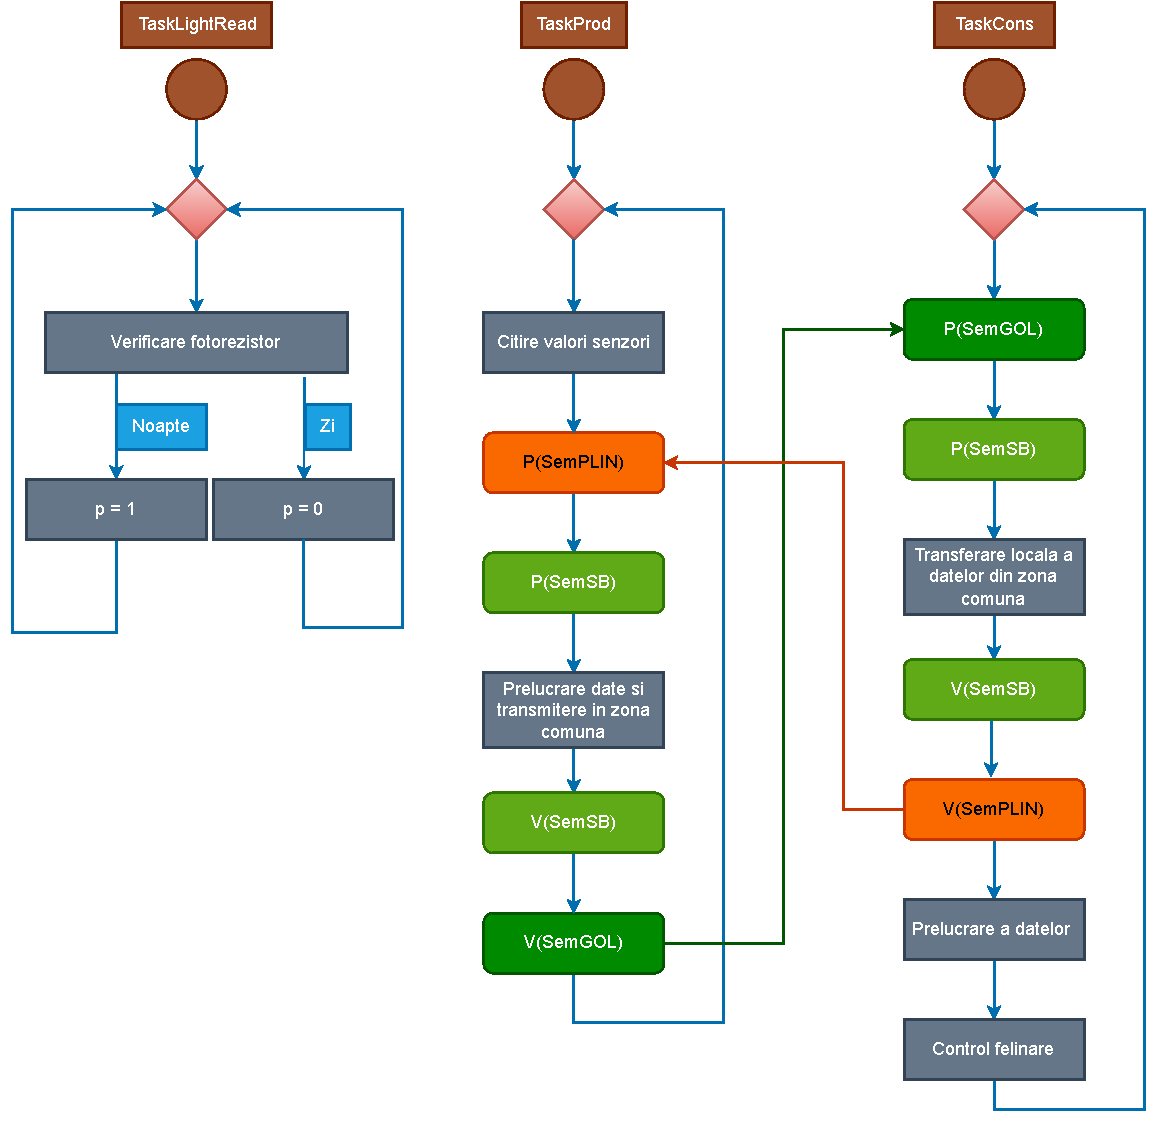
\includegraphics[width=0.9\linewidth,keepaspectratio]{pics/diag2.drawio.pdf}
    \end{center}
    \caption{Diagramă task-uri pentru funcționare pe timp de zi}
    \label{fig:dtask2}
\end{figure}

Pe urmă, trebuie aduse modificări structurii task-urilor, iar acestea sunt ilustrate în \figref{fig:dtask2}. TaskLightRead nu mai reinițializează valorile variabilelor, ci doar modifică valoarea unei variabile $p$. Aceasta îndeplinește rolul de flag, pentru a determina dacă este zi sau noapte. Dacă valoarea sa indică faptul că este zi, partea de \emph{Control felinare} din TaskCons va egala cu 0 valorile din vectorul de luminozitate, pentru stingerea \textbf{completă} a acestora.

\section{Avantaje dublare senzori}
Dublarea senzorilor constă în folosirea a doi senzori de prezență pe porțiunea de drum în care, în mod normal, aș fi folosit unul singur. În funcție de distanța dintre ei și de modul în care sunt utilizate datele citite, aceștia pot îndeplini mai multe scopuri. 

\subsection{Creșterea vitezei maxime la care poate fi detectat un vehicul} \label{speed}
Majoritatea elementelor adiționale adăugate sistemului vor duce la scăderea frecvenței citirii senzorilor de prezență, ceea ce poate cauza trecerea neobservată a vehiculelor, fenomen explicat în \autoref{time}. 

Problema poate fi rezolvată prin înlocuirea fiecărui senzor cu o grupare de doi senzori aflați la distanța $k$ între ei. În această situație, distanța pe care trebuie să o parcurgă un vehicul în intervalul de timp dintre două citiri ale senzorilor, pentru a nu fi detectat, crește cu o valoare egală cu $k$.

În \figref{fig:double} este ilustrat cazul unui vehicul ce nu a fost văzut de primul senzor, dar următoarea citire a avut loc înainte ca acesta să-l depășească și pe al doilea.
\begin{figure}[!ht]
    \begin{center}
    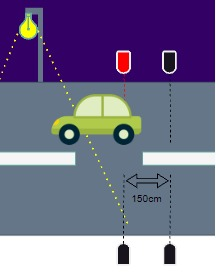
\includegraphics[width=0.3\linewidth,keepaspectratio]{pics/double.jpg}
    \end{center}
    \caption{Creșterea vitezei maxime la care poate fi detectat un vehicul, prin dublarea senzorilor}
    \label{fig:double}
\end{figure}
În acest caz, considerând $k=150$cm și citirea senzorilor la fiecare 85 ms, viteza maximă cu care un vehicul cu lungimea de 190cm poate să se deplaseze fără să fie vreodată neobservat crește de la 80.47 km/h la 144km/h. Counter-ul ce determină aprinderea următorului felinar se va comporta la fel ca în situația activării primului senzor, dar se va stoca într-o variabilă de tip flag care dintre senzori au fost activați, pentru a ajusta distanța folosită la calcularea vitezei.

\subsection{Permiterea funcționării sistemului în ambele sensuri de circulație} \label{rev}
Un alt lucru făcut posibil de dublarea senzorilor este identificarea sensului de deplasare al unui vehicul. În continuare este prezentat cazul unei străzi cu două benzi și sensuri opuse de circulație. În \figref{fig:dep1} este prezentat momentul depășirii unui senzor de un vehicul aflat pe sensul său de circulație, iar \figref{fig:dep2} este reprezentarea aceluiași vehicul în urma trecerii pe contrasens, în cazul unei depășiri. 
\begin{figure}[!ht]
    \begin{center}
    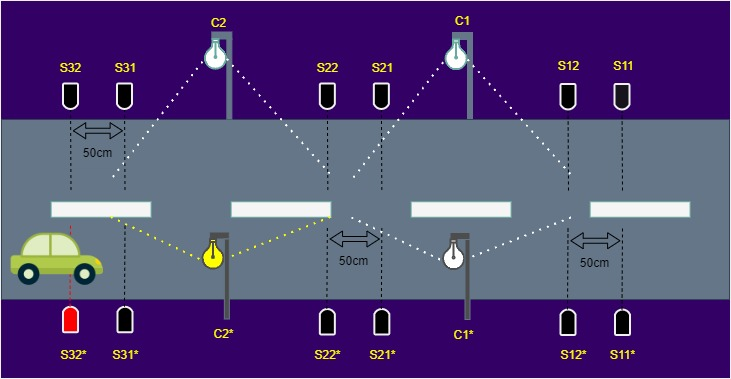
\includegraphics[width=\linewidth,keepaspectratio]{pics/dep1.jpg}
    \end{center}
    \caption{Sistem funcțional pentru ambele sensuri de circulație, moment 1}
    \label{fig:dep1}
\end{figure}

\begin{figure}[!ht]
    \begin{center}
    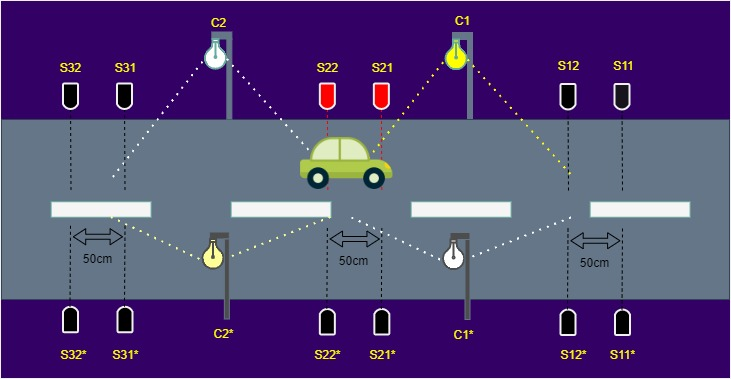
\includegraphics[width=\linewidth,keepaspectratio]{pics/dep2.jpg}
    \end{center}
    \caption{Sistem funcțional pentru ambele sensuri de circulație, moment 2}
    \label{fig:dep2}
\end{figure}

Primul senzor întâlnit în fiecare pereche pe sensul normal ar circulației(S11, S21, S31, S32*, S22*, S12*) este folosit pentru incrementarea sau decrementarea variabilelor counter $\mathbf{c}$ și pentru măsurarea vitezei automobilului, iar valoarea citită de cel de-al doilea(S12, S22, S32, S31*, S21*, S11*) are rolul de a stabili sensul de deplasare. Deoarece înregistrarea momentului de timp la care un vehicul depășește un senzor se face doar la modificarea valorii citită de la acesta (ref), pot verifica tot atunci valoarea citită de la senzorul ajutător. Dacă  aceasta indică prezența unui obiect, înseamnă că vehiculul se află pe contrasens. În această situație, se întâmplă următoarele:

\begin{enumerate}
    \item Se incrementează un element al unui counter $\mathbf{cs}$, corespunzător grupării de senzori (S21-S22).
 \item Se verifică starea counter-ului grupării de senzori anterioare, relativ la sensul de deplasare al vehiculului, pe același sens (în acest caz, S31-S32, și egal cu 0). Dacă aceasta este:
 \begin{itemize}
     \item egală cu 0 - ultimul senzor depășit de vehicul a fost pe cealaltă bandă, deci se decrementează $\mathbf{c}$ pentru cel mai apropiat felinar de pe acea bandă (aici, C2*) 
     \item mai mare ca 0 - ultimul senzor depășit de vehicul a fost pe aceeași bandă deci se decrementează $\mathbf{c}$ pentru cel mai apropiat felinar depășit de acesta (aici, C2).   
 \end{itemize}
 \item Se incrementează elementul counter $\mathbf{c}$ pentru stâlpul următor(C1).
 \item Se decrementează valoarea $\mathbf{cs}$ analizată mai sus în urma calculului vitezei, dacă aceasta este mai mare ca 0.
\end{enumerate}

Este important să fie cunoscut sensul de circulație pe care se află vehiculul la depășirea senzorului anterior până la momentul calcului vitezei, deoarece trecerea pe celălalt sens duce la schimbarea valorii  folosite pentru distanța dintre senzori. Noua distanță \textit{d'} este reprezentată în \figref{fig:dist} și, cunoscând lățimea \textit{w} a drumului, se află prin: 
\be
\label{eq:test}
d'=\sqrt{(w/2)^2+(d+50cm)^2}
\ee
\begin{figure}[!ht]
    \begin{center}
    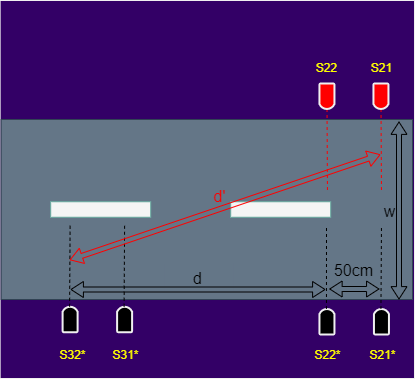
\includegraphics[width=0.4\linewidth,keepaspectratio]{pics/dist.png}
    \end{center}
    \caption{Noua distanță folosită la calcularea vitezei}
    \label{fig:dist}
\end{figure}

O problemă ce trebuie rezolvată pentru implementarea unui astfel de sistem este calculul distanței optime dintre senzorii ce aparțin aceleiași perechi. Aceasta trebuie să fie cât mai mică posibil, pentru a asigura imposibilitatea unui vehicul de a activa doar unul dintre senzori la trecerea pe contrasens. În același timp, ea trebuie să fie și destul de mare pentru ca vehiculul să nu aibă timp să ajungă la al doilea senzor din pereche, înainte să fie detectat de primul, pe sensul normal de mers. În ambele cazuri negative, rezultatul este incrementarea counterului $\mathbf{c}$ al felinarului din spatele vehiculului, în loc de cel din fața sa. Pentru folosirea unei distanțe destul de mici între senzori, este nevoie de o frecvență mare a citirilor, sau de implementarea sistemului pe drumuri cu limite legale mici pentru viteza de circulație.


\section{Soluție implementare sistem pentru cazul unei autostrăzi} \label{hw}

Pentru abordarea cazului implementării sistemului în timp real pe o autostradă cu 4 benzi de circulație(2 pentru fiecare sens, cu separare la mijloc), trebuie rezolvate următoarele probleme:
\begin{itemize}

\item Vitezele mai mari aduc și erori mai mari în măsurarea lor, conform analizei realizate în \autoref{fail}.

\item Vehiculele pot atinge viteze care le permit depășirea neobservată a senzorilor.

\item Variabilele counter din $\mathbf{c}$ pot să primească valori greșite în momentul trecerii a două mașini în paralel.

\item Aprinderea unui singur felinar în fața unui vehicul ce se deplasează cu 130-140 km/h poate fi deranjant pentru ochii șoferului și poate cauza accidente din cauza vizibilității scăzute.
 
\end{itemize}
Soluția propusă de mine constă în câteva modificări aduse sistemului, în starea sa inițială, pentru a rezolva aceste probleme.

În primul rând, toți senzorii de prezență vor fi dublați, pentru creșterea vitezei maxime la care un vehicul poate fi detectat, ca în \autoref{speed}. Apoi, este dublată distanța dintre aceste grupări, pentru a mări precizia cu care este calculată viteza. În  \figref{fig:hw1}, \figref{fig:hw2} și \figref{fig:hw3} sunt surprinse trei momente de interes din trecerea unui vehicul prin sistem. Fiecare senzor din aceste imagini reprezintă, în realitate, câte o pereche de senzori pe care le voi numi, pentru restul secțiunii, grupuri. Pentru a număra corect automobilele din fiecare porțiune a drumului, se folosește câte un grup pentru fiecare bandă de circulație, amândouă influențând valoarea counter-ului $\mathbf{c}$ corespunzător acelorași felinare. Problema vizibilității poate fi rezolvată prin asigurarea faptului că un automobil va avea în orice moment cel puțin două felinare aprinse în fața sa.
\begin{figure}[!ht]
    \begin{center}
    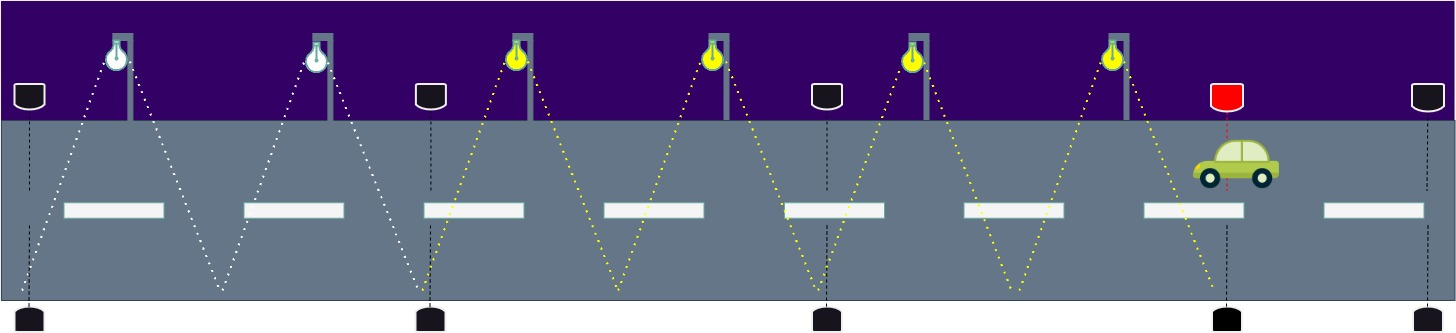
\includegraphics[width=\linewidth,keepaspectratio]{pics/hw1.jpg}
    \end{center}
    \caption{Model sistem autostradă, moment 1}
    \label{fig:hw1}
\end{figure}

\begin{figure}[!ht]
    \begin{center}
    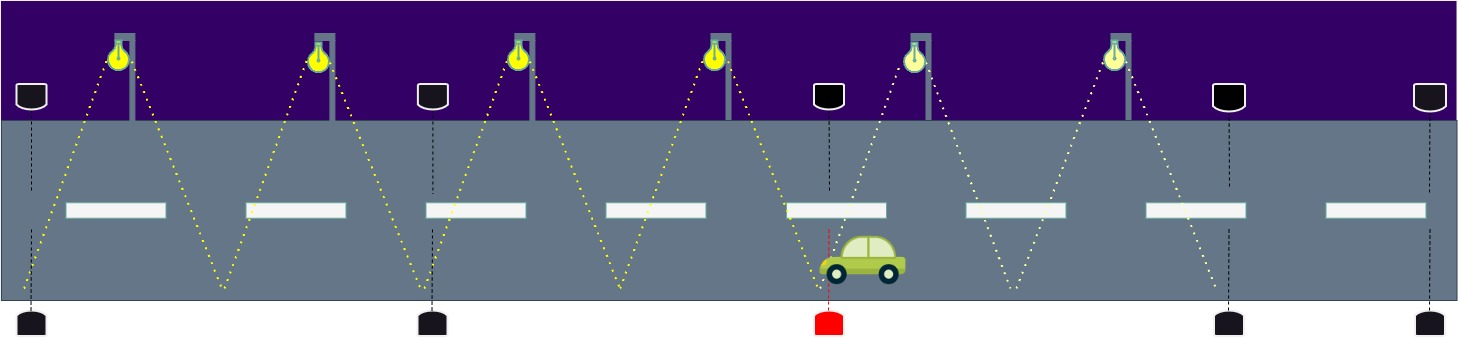
\includegraphics[width=\linewidth,keepaspectratio]{pics/hw2.jpg}
    \end{center}
    \caption{Model sistem autostradă, moment 2}
    \label{fig:hw2}
\end{figure}

\begin{figure}[!ht]
    \begin{center}
    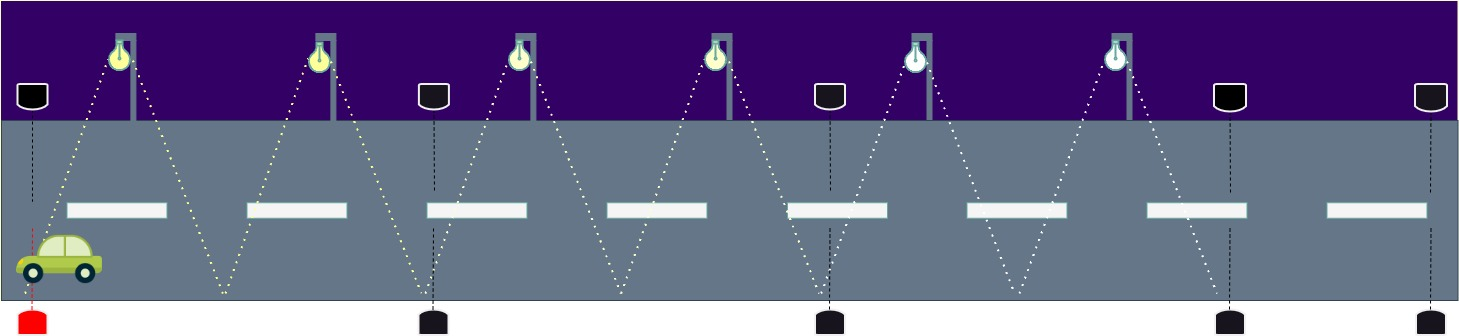
\includegraphics[width=\linewidth,keepaspectratio]{pics/hw3.jpg}
    \end{center}
    \caption{Model sistem autostradă, moment 3}
    \label{fig:hw3}
\end{figure}

 După cum este prezentat în imagini, la momentul depășirii unui grup, cele 2 felinare din urma acestuia se vor stinge, următoarele două vor rămâne aprinse, iar al 3-lea și al 4-lea după acesta se vor aprinde. 
 
 Din moment ce felinarele funcționează în grupuri de câte două, și dimensiunea vectorului $\mathbf{c}$ poate fi înjumătățită. 
 Nu este necesar a fi luat în calcul cazul circulației în sens opus, deoarece pe fiecare bandă a autostrăzii sensul este unic. Astfel, o versiune identică a sistemului poate fi instalată și pentru celelalte două benzi.


\chapter{Dezvoltări ulterioare și posibile limitări}
\label{chap:next}
Ca scopuri pentru dezvoltarea ulterioară a proiectului pot menționa testarea și implementarea ideilor din \autoref{chap:extra}, dar și rezolvarea problemelor cărora nu le-am găsit încă o soluție.
\section{Problema numărării vehiculelor pe străzi cu mai multe benzi de circulație}
Una dintre aceste probleme este activarea senzorilor la momentul trecerii unui vehicul pe cealaltă banda de circulație. În exemplul din \figref{fig:dezv}, aplicat modelului din \autoref{hw}, vehiculul ar incrementa counter-ul corespunzător următoarelor felinare de 2 ori cu o singură trecere.
 
\begin{figure}[!ht]
    \begin{center}
    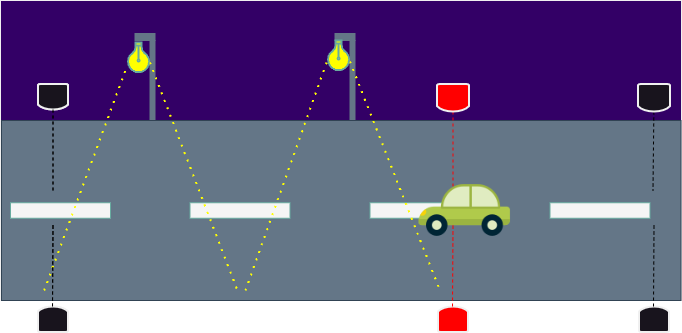
\includegraphics[width=0.6\linewidth,keepaspectratio]{pics/dezv.png}
    \end{center}
    \caption{Activare simultană a 2 senzori}
    \label{fig:dezv}
\end{figure}

 Data viitoare când acesta se află în întregime pe o singură bandă, el va decrementa counter-ul din urmă doar cu 1, iar consecința va fi o desincronizare dintre valorile din counter și numărul real de vehicule de pe stradă (rezultat asemănător și în cazul situației din \autoref{rev}).  Nici micșorarea razei de detecție a senzorilor nu rezolvă această problemă, deoarece sunt create situații în care un vehicul poate trece prin mijlocul drumului complet neobservat, cauzând aceeași desincronizare menționată anterior. Aici m-am gândit la suplimentarea cu metode de măsurat a distanței de la senzori, prin adăugarea, de exemplu, a senzorilor ultrasonici menționați în \autoref{collect}. Un dezavantaj este faptul că nu am lucrat cu astfel de senzori, deci nu cunosc toate limitările ce pot fi întâlnite în practică. 

Problema numărării vehiculelor apare și în cazul străzilor cu mai mult de 2 benzi pe același sens de circulație, deoarece 2 astfel de senzori plasați pe părți opuse ale străzii nu pot diferenția între 2 sau mai multe automobile care trec în același timp. 


\section{Problema calculării vitezei pe străzi cu mai multe benzi de circulație}


Pe orice stradă pe care este posibilă depășirea vehiculelor, calculul vitezei devine greu de realizat, deoarece acesta se realizează cu presupunerea că primul vehicul care intră într-o porțiune de drum va fi și primul care iese din ea. Aceasta este, în opinia mea, cea mai mare limitare a sistemului în starea sa actuală. În schimb, chiar și în cazul eliminării componentei de măsurat viteza, performantele obținute ar fi, în continuare, satisfăcătoare din punct de vedere al consumului de energie electrică. Pentru studiul din \cite{7513906}, unde consumul pe durata unei luni a scăzut cu 40\%, felinarele funcționează la intensitate maximă la detecția unui vehicul, indiferent de viteza acestuia.

 \section{Caz particular pietoni}

Detecția pietonilor poate fi considerată un caz particular de stradă cu mai multe benzi de circulație.  Principalele diferențe sunt dificultatea în a determina comportamentul acestora și faptul că viteza lor nu este la fel de relevantă ca cea a vehiculelor. Senzorii pentru prezență destinați detectării pietonilor trebuie să fie separați de cei pentru automobile, pentru a nu influența măsurarea vitezei acestora, ca în \figref{fig:ped}. 
 \begin{figure}[!ht]
    \begin{center}
    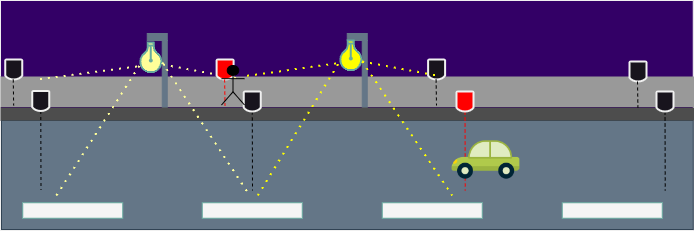
\includegraphics[width=0.8\linewidth,keepaspectratio]{pics/ped.png}
    \end{center}
    \caption{Sugestie sistem pentru detectarea pietonilor}
    \label{fig:ped}
\end{figure}

Direcția deplasării pietonilor nu poate fi prezisă cu certitudine. Aceștia se pot și opri sau părăsi drumul, de exemplu pentru a intra într-o clădire. De aceea, sunt de părere că trecerea pietonilor nu ar trebui să influențeze counter-ul ce determină funcționarea felinarelor, ci doar să aprindă cele două sau mai multe felinare din jurul senzorului activat, la intensitate medie, în cazul în care acestea nu erau deja aprinse. Pentru această metodă, este necesară adăugarea unui timer(\ref{timer}) , care să determine stingerea felinarelor la trecerea unei perioade de timp prestabilite.

\section{Utilizare timere} \label{timer}

Arduino IDE permite folosirea unor funcții specializate pentru realizarea operațiilor cu momente de timp, prin adăugarea de biblioteci ce se bazează pe funcțiile millis() sau micros(). Atât folosirea unor timere ca unică metodă de control a stingerii felinarelor, cât și îmbinarea unui astfel de element cu sistemul realizat, poate oferi performanțe mai bune în cazurile limită. Aceasta pare a fi chiar obligatorie pentru orice fel de astfel de sistem care are ca scop și detectarea pietonilor. În metoda mea de implementare am preferat să nu adaug timere, pentru a evidenția cât mai mult răspunsurile sistemului la stimuli externi, specifice unui sistem în timp real. 

Un exemplu de posibilă îmbunătățire adusă de adăugarea unui timer este decrementarea automată a counter-ului $\mathbf{c}$ pentru o anumită porțiune de drum, la trecerea unei perioade de timp prestabilită de la ultima dată când a intrat un vehicul în ea. Aceasta ar duce la stingerea felinarului în cazul în care un vehicul se oprește între 2 senzori, sau dacă acesta, din posibile erori hardware, nu este detectat de senzorul de la ieșirea din porțiunea respectivă. 

\chapter{Concluzie}
\label{chap:fin}

Pe parcursul lucrării nu am adus în evidență foarte mult potențialul câștig al sistemului din punct de vedere al reducerii consumului de energie electrică și a emisiilor de dioxid de carbon(CO2), ci am insistat mai mult pe implementarea în sine și pe limitările întâlnite în practică. 

Am identificat elementele hardware necesare și am prezentat o metodă de implementare funcțională pentru un caz restrâns. Prin analiza realizată anterior am demonstrat că majoritatea acestor limitări sunt cauzate de calculul vitezei vehiculelor, pe tipuri de drum unde comportamentul acestora este imprevizibil. De aceea, o metodă de implementare similară și-ar putea avea locul în cazul străzilor cu sens unic, sau cu o singură bandă de circulație pentru fiecare sens, cu mențiunea că integrarea unor componente ce permit măsurarea distanței sau renunțarea în întregime la calculul vitezei ar putea deschide calea mai multor posibilități de utilizare. 


Sunt de părere că implementarea unui astfel de sistem, în urma tratării cazurilor limită, oferă cel puțin condiții necesare siguranței rutiere, cu potențiale câștiguri la costurile operaționale, în funcție de densitatea traficului pe timpul nopții pe drumurile unde ar fi folosit. 

Prin urmare, consider că un astfel de sistem ar putea fi implementat prin generalizarea soluției identificate.
%%%%%%%%%%%%%%%%%%%%%% back matter %%%%%%%%%%%%%%%%%%%%%%%%%%%%%%%%%%%%%%
\appendix
\appendixpage
\addappheadtotoc
\begin{appendices}																				  % from here onwards are the appendices
% fisiere sursa

\chapter{Fișiere sursă}
\label{chap:sources}

\section{TaskProd} \label{tp}
\begin{verbnobox}[\verbarg]
 void TaskProd( void *pvParameters __attribute__((unused)) )  
{
  for (;;) 
  { 
    xSemaphoreTake(SemNOAPTE, portMAX_DELAY);

    bc[0] = digitalRead(49);
    bc[1] = digitalRead(50);
    bc[2] = digitalRead(51);
    bc[3] = digitalRead(52);
    bc[4] = digitalRead(53);

    xSemaphoreTake(SemPLIN,portMAX_DELAY);
    xSemaphoreTake(SemSB,portMAX_DELAY);

     for(int in = 0; in < 5; in ++){
        if (f[in] == 1){
          b[in]= bn[in];
          bn[in] = 0;
          f[in] = 2;
        }
        if (aux[in] - bc[in] == 1) {
            if (in <= 3) {
              c[in] ++;
            }
            if ((in >= 1) && c[in-1]>0){
              c[in - 1] --;
             if ((bn[in-1] != 0) &&(c[in - 1] == 1)){
                  f[in-1] = 1;
               } 
           }      
            if (in == 4)
              b[in] = millis();
            else if ((in <= 3) && (c[in] == 1)){ 
                  b[in] = millis();
            }
            else if ((in <= 3) && (c[in] > 1)){
                bn[in] = millis();
            }
         }
          aux[in] = bc[in];      
      }
          xSemaphoreGive(SemSB);
          xSemaphoreGive(SemGOL);
        
          vTaskDelay(1);  
   }
}   
\end{verbnobox}

\section{TaskCons} \label{tc}
\begin{verbnobox}[\verbarg]
void TaskCons( void *pvParameters __attribute__((unused)) )  
{
  for (;;)
  {

    xSemaphoreTake(SemGOL, portMAX_DELAY);
    // Transfer date buffer
    xSemaphoreTake(SemSB, portMAX_DELAY);
    for (int i = 0; i < 5; i ++) { 
      z[i] = b[i];
      zn[i] = bn[i];
    }

    xSemaphoreGive(SemSB);
    xSemaphoreGive(SemPLIN);
    //  CALCULE
    for (int i = 0; i < 4; i ++) {
      if (i==3)
        t[i] = z[i + 1] - z[i];
      else if (c[i + 1] == 1)
        t[i] = z[i + 1] - z[i];
      else if (c[i + 1] == 2)
        t[i] = zn[i + 1] - z[i];
      
      if (t[i] != 0)
        vint[i] = 10*d * 3.6/((float)t[i]);
      else if (t[i] == 0) 
        vint[i] = 0;
      if (auxv[i] != vint[i]){
        if ((f[i] != 2)&&(vint[i]>=0)){
          v[i] = vint[i];
          Serial.print("  t[");Serial.print(i);Serial.print("] = ");
          Serial.print(t[i]);
          Serial.print("  ||||");
          for (int j = 0; j < 4; j ++) {
            if (j==i){
              Serial.print("<v[");Serial.print(j);Serial.print("] = ");
              Serial.print(v[j]);
              Serial.print(">");
            }
            else {
              Serial.print(" v[");Serial.print(j);Serial.print("] = ");
              Serial.print(v[j]);     
              Serial.print(" ");
            }
           }
        Serial.println("");
        }
        else {Serial.print("  z[");Serial.print(i);Serial.print("] = ");
          Serial.print(z[i]);
          Serial.print("  zn[");Serial.print(i);Serial.print("] = ");
          Serial.print(zn[i]);
          Serial.print("  z[");Serial.print(i+1);Serial.print("] = ");
          Serial.print(z[i+1]);
          Serial.print("  zn[");Serial.print(i+1);Serial.print("] = ");
          Serial.print(zn[i+1]);
          Serial.print("  t[");Serial.print(i);Serial.print("] = ");
          Serial.print(t[i]);
          Serial.print(" ***");
        Serial.println("");
          f[i] = 0;
        }
      }  
      auxv[i] = vint[i];
      
      if (i > 0){ 
        if (lum[i - 1] < 3)
          lum[i - 1] = 3;
        if ((c[i] == 0) && ( lum[i - 1] > 3)) {
            if (timp == 0) {
              if (lum[i - 1] > 8)
                lum[i - 1] = lum[i - 1] * 0.7;
              else
                lum[i - 1] --;
            }
            timp ++;
            timp = timp % 5;      
        }
        else if (c[i] == 0) {     
        }
        else if (c[i] == 1){
          if (v[i-1] > 4){ 
            lum[i - 1] = 255;      
          }
          else if (v[i-1] > 1){ 
             if (lum[i - 1] > 150)
               lum[i - 1] =  lum[i - 1] - 2;
             else 
               lum[i - 1] = 150;
          }           
          else if (v[i-1] > 0){ 
             if (lum[i - 1] > 40)
               lum[i - 1] =  lum[i - 1] - 2;
             else 
               lum[i - 1] = 40;
          }
         }
         else if (c[i] == 2){
          if ((v[i-1] > 4)&& (lum[i - 1] < 150)){ 
            lum[i - 1] = 255;      
          }
          else if ((v[i - 1] > 1) && (lum[i - 1] < 150)){ 
            lum[i - 1] = 150;
          }           
         }  
         analogWrite(4 + i, lum[i - 1]);  
      }
   }
  }
}
\end{verbnobox}
\section{TaskLightRead} \label{tlr}
\begin{verbnobox}[\verbarg]
void TaskLightRead( void *pvParameters __attribute__((unused)) ) 
{

  for (;;)
  {
    int FotoRez = analogRead(A0);
      if (FotoRez>80)
        xSemaphoreGive( SemNOAPTE );
      else {
        Serial.println(FotoRez);
        analogWrite (5, 0);
        analogWrite (6, 0);
        analogWrite (7, 0);
        timp = 0;
        b[0] = 0; b[1] = 0; b[2] = 0; b[3] = 0; b[4] = 0;
        f[0] = 0; f[1] = 0; f[2] = 0; f[3] = 0; f[4] = 0;
        bn[0] = 0; bn[1] = 0; bn[2] = 0; bn[3] = 0; bn[4] = 0;
        c[0] = 0; c[1] = 0; c[2] = 0; c[3] = 0;
        lum[0] = 0; lum[1] = 0; lum[2] = 0;
        v[0] = 0; v[1] = 0; v[2] = 0; v[3] = 0;
        vint[0] = 0; vint[1] = 0; vint[2] = 0; vint[3] = 0;
        t[0] = 0; t[1] = 0; t[2] = 0; t[3] = 0;
        aux[0] = 0; aux[1] = 0; aux[2] = 0; aux[3] = 0; aux[4] = 0;
        auxv[0] = 0; auxv[1] = 0; auxv[2] = 0; auxv[3] = 0;
      }
  }
}
\end{verbnobox}

\section{TaskLCD} \label{tlcd}

\begin{verbnobox}[\verbarg]
void TaskLCD( void *pvParameters __attribute__((unused)) )  
{
  for (;;)
  {
    if (p == 0) {
      lcd.begin(16, 2);
    lcd.setBacklight(255);
    lcd.home(); 
    lcd.clear();
      p = p + 1;
    }
    xSemaphoreTake(SemLCD, portMAX_DELAY);
    xSemaphoreTake(SemSB, portMAX_DELAY); 
      lcd.clear();
      for (int i = 0; i < 4; i ++){
      if (i == 0)
        lcd.setCursor(0, 0);
      else if (i == 1)
        lcd.setCursor(7, 0);
      else if (i == 2)
        lcd.setCursor(0, 1);
      else if (i == 3)  
        lcd.setCursor(7, 1);
      lcd.print(v[i]);

  }
      lcd.print(" km/h");
      xSemaphoreGive(SemSB);
  }
}
\end{verbnobox}
\end{appendices}

\cleardoublepage

\printbibliography[heading=bibintoc]
\section*{Lista contribuțiilor personale}
\begin{table}[ht!]
\begin{tabular}{|c|c|c|}
\hline
\multicolumn{3}{|c|}{\textbf{Sistem în timp real pentru controlul iluminatului public}} \\
\multicolumn{3}{|c|}{\textbf{Durbală Cristian}} \\
\multicolumn{3}{|c|}{\textbf{Prof. dr. ing. Monica Drăgoicea}} \\
\hline
 & Activitate & Durată [zile] \\
\hline
1 & Documentare & 5  \\
\hline
 2 & Testare componente hardware & 0.5\\
\hline
3 & Alegere și implementare soluție hardware & 3\\
\hline
4 & \begin{tabular}[c]{@{}c@{}}Implementare cod - aprindere felinare pe baza counter-ului\\ de obiecte\end{tabular} & 1.5 \\
\hline
5 & Redactare lucrare - Introducere și elemente hardware & 2 \\
\hline
6 & \begin{tabular}[c]{@{}c@{}} Implementare cod - realizare calcul viteză\\ pentru 1 vehicul și aprinderea felinarelor în funcție de aceasta\end{tabular} & 0.5\\
\hline
7 & Implementare cod - realizare calcul viteză pentru 2 vehicule & 3\\
\hline
8 & Redactare lucrare - restul lucrării & 4 \\
\hline
\end{tabular}
\centering
\label{tab:lista_contrib}
\end{table}
\end{document}